\documentclass[a4paper,10pt]{scrartcl}
\usepackage{mathe-vorlesung}
\usepackage{graphicx}
\renewcommand{\equiv}{\Longleftrightarrow}
\newcommand{\eps}{\varepsilon}
\newcommand{\del}{\delta}
\newcommand{\homo}{\cong}
\usepackage{txfonts}
\renewcommand{\bigsqcap}{\prod}

\title{Topologie}

\begin{document}

\maketitle

\tableofcontents
\newpage
\begin{center}
\LARGE\textbf{Vorwort}
\end{center}
\begin{seg}{Was ist Topologie?}
\begin{itemize}
\item "` Unterzeichnung geometrischer Objekte bis auf stetige Dekorationen. "'
\item "` Stetigkeitsgeometrie"', "` qualitative Geometrie "', "`Gummi-Geometrie"'
\end{itemize}
Objekte werden in der Topologie als gleich angesehen, wenn sie durch eine in beiden Richtungen stetige bijektive Abbildung aufeinander abgebildet werden kann ("` Homöomorphismus"').
\end{seg}
So zum Beispiel für Teilmengen des $\R^2$:
\begin{figure}[h]
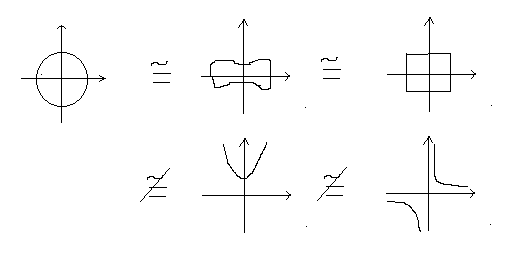
\includegraphics[scale=0.7]{fig1.png}
\end{figure}
\begin{ex*} 
Topologische Begriffe sind beispielsweise \emph{Stetigkeit, offene/abgeschlossene Mengen, Umgebung, Rand, Abschluss, Konvergenz, kompakt, zusammenhängend, Homotopie}.  Die konkreten Definition werden im Verlauf dieser Vorlesung geklärt.
\end{ex*}
\section{Grundbegriffe}
\subsection{Metrische und topologische Räume}
\begin{df}
Ein \emph{metrischer Raum} ist eine Menge $X$ zusammen mit einer Funktion $d: X \times X \rightarrow \R$, genannt Metrik oder \emph{Abstandsfunktion}, so dass folgende Axiome gelten:
\begin{enumerate}[(\roman{enumi})]
\item \emph{Positivität}: $d(x,y)\ge 0 \land d(x,y)=0\equiv x=y$
\item \emph{Symmetrie}: $d(x,y)=d(y,x)$
\item \emph{Dreiecksungleichung}: $d(x,z) \le d(x,y)+d(y,z)$
\end{enumerate}
\end{df}
\begin{ex*}
Auf $\R^n$ ist durch die \emph{Euklidische Norm} $|x|=\sqrt{x_1^2+...+x_n^2}$ die \emph{Euklidische Abstandsfunktion} $d(x,y)=||x-y||$ gegeben. Auf $\R$ oder auf $\C$ ist diese Metrik durch den Betrag $d(x,y):=|x-y|$ definiert.  Man erhält auf diese Weise aus jeder Norm eine Metrik. Hierbei liefern verschiedene Normen natürlich verschiedene Metriken. Hier einige Beispiele auf $\R^2$:
\begin{itemize} 
\item euklidische Norm: $||x||_2=\sqrt{x_1^2+x_2^2}$
\item Maximumsnorm: $||x||_\infty := \max(|x_1|, |x_2|)$
\item $\Eins$-Norm $||x||_1 := |x_1|+|x_2|$
\end{itemize}
\end{ex*}

\begin{ex*}
Die diskrete Metrik definiert durch:
\[
d(x,y)=\begin{cases}
  0, & \text{falls} x=y \\ 1, & \text{falls} x\neq y
\end{cases}
\]
\end{ex*}

Es lassen sich zwei zentrale mathematische Begriffe mit HIlfe von Abstandsfunktionen definieren:
\begin{itemize}
\item Konvergenz von Folgen
\item Stetigkeit von Abbildungen
\end{itemize}

\begin{df}[Konvergenz im metrischen Räumen]
Sei $X$ ein metrischer Raum und $x_N, n\in \N$ eine Folge in $X$. Wir sagen $(x_n)_{n\in \N}$ \emph{konvergiert}, falls es ein $a \in X$ gibt, so dass gilt:
\[
\forall_{\varepsilon>0}\exists_{k\in\N}\forall_{n\ge k}: d(x_n,a)<\varepsilon
\]
\end{df}
In diesem Fall sagen wir, $a$ ist der \emph{Limes} (oder Grenzwert) von $(x_n)_{n\in \N}$ (und schreiben $x_n\rightarrow a, \lim\limits_{n\rightarrow \infty} x_n=a$) 

\begin{st} 
In einem metrischen Raum ist der Limes eine konvergente Folge eindeutig bestimmt.
\end{st}
\begin{proof}
Seien $a$ und $b$ Limiten von $(x_n)_{n\in \N}$ mit $\delta := d(a,b)>0$.

Da $(x_n)_{n\in \N}$ gegen $a$ konvergiert, gibt es $k\in \N$, sodass $d(x_n,a)<\frac{\delta}{2}$ für alle $n \ge k$.
Dann gilt nach Dreiecksungleichung:
\[
\delta=d(a,b)\le \underbrace{d(x,x_n)}_{<\frac{\delta}{2}}+d(x_n,b)
\]
Also gilt $d(x_n,b)\ge \frac{\delta}{2}$ für alle $n\ge b$, was der Konvergenz gegen $b$ widerspricht.
\end{proof}
\begin{df}[$\eps$-$\delta$-Definition der Stetigkeit in metrischen Räumen]
Seien $X$ und $\tilde X$ metrische Räume mit Abstandsfunktion $d$ bzw. $\tilde d$. Eine Abbildung $f: X \rightarrow \tilde X$ heißt stetig in$x \in X$ falls gilt: 
\[\forall_{\eps>0}\exists_{\delta>0} \forall_{x'\in X}: d(x,x')<\delta \implies \tilde d(f(x), f(x'))<\eps\]

Die Abbildung heißt \emph{stetig}, falls dies für alle $x\in X$ gilt.  Stetigkeit in metrischen Räumen hängen eng zusammen. Es gilt:
\end{df}
\begin{st}
Eine Abbildung $f: X\rightarrow \tilde X$ zwischen metrischen Räume ist genau dann stetig, wenn für jede konvergente Folge $x_n \rightarrow a$ in X gilt, dass $f(x_n) \rightarrow f(a)$
\end{st} 
\begin{proof}
\begin{seg}{"`$\implies$"'}
Sei $\eps>0$, dann gibt es $\delta>0$, so dass aus $d(x',a)<\delta$ folgt: $d(f(x'),f(a))<\eps$. Weiter gibt es ein $k\in \N$, so dass $d(x_N,a)y\delta$ für $n \ge k$.  Insgesamt folgt $d(f(x_n),f(a))<\eps$ für alle $n\ge k$.
\end{seg}
\begin{seg}{"`$\Longleftarrow$"'}
Angenommen, $f$ ist nicht stetig. Dann gibt es ein $x \in X$ und ein $\eps>0$, so dass es zu jeden $n\in \N$ ein $x$ mit $d(x_n,x)<\frac{1}{n}$ und $d(f(x_1), f(x))\ge \eps$ gibt. Damit ergibt sich der Widerspruch.
\end{seg}
\end{proof}
Die obigen Definition lassen sich mit Hilfe von $\eps$-Bällen umformulieren:
\begin{df}
Sei $X$ ein metrischer Raum und $x\in X$, dann heißt die Teilmenge 
\[
B_\eps(x)={x'\in X|d(x',x)<\eps}
\]
von $X$ heißt der (\emph{offene}) \emph{Ball mit Radius $\eps$ um x} (kurz: \emph{$\eps$-Ball}).
\end{df}
\begin{df}
In einem metrischen Raum heißt eine Teilmenge $U\subset X$ \emph{offen}, wenn es um jeden ihrer Punkte einen offenen $\eps$-Ball gibt, der ganz in U enthalten. Eine Teilmenge A heißt \emph{abgeschlossen}, wenn ihr Komplement $X\setminus A$ offen ist.  Eine Teilmenge $U \subset Y$ heißt \emph{Umgebung} eines Punktes $ x\in X$, falls es eine offene Teilmenge $V \subset X$ gibt mit $x\in v$ und $V \subset U$.  (Äquivalent: falls es ein $\eps$ mit $B_\eps(x)\subset U$ gibt.  
\end{df}

\begin{figure}[h]
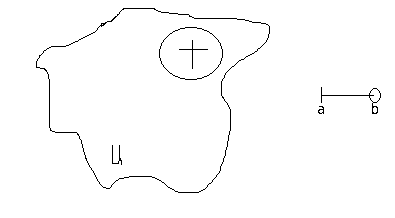
\includegraphics[scale=0.5]{fig3.png}
\end{figure}

Konvergenz und Stetigkeit lassen sich in metrischen Räumen durch offene Mengen beschreiben.
\begin{st}
In einem metrischen raum konvvergiert eine Folge $(x_n)_{n \in \N}$ genau dann gegen x, wenn es zu jeder Umgebung $U$ von $x$ ein $k \in \N$ gibt, so dass $x_n \in U$ für alle $n \ge k $ gilt.\\
\underline{Kurz:} Eine Folge $(x_n)_{n \in \N}$ konvergiert gegen $x$, wenn in jeder Umgebunng von $x$ \emph{fast alle} ($\hat =$ alle bis auf endlich viele) Folgenglieder liegen.
\end{st}
\begin{proof}
Die Äwuivalenz gilt, da jede Umgebung von $x$ einen $\eps$-Ball um $x$ enthält und umgekehrt jeden $\eps$-Ball um $x$ auch eine Umgebung von $x$ ist.
\end{proof}
\begin{st}\label{st:1.8}
Eine Abbildung zwischen metrischen Räumen $f: X\rightarrow \tilde X$ ist genau dann stetig in $x \in X$, wenn es zu jeder Umgebung $V$ von $f(X)$ eine Umgebung $U$ von $x$ gibt, so dass U unter $ f $ in V abgebildet wird; oder äquivalent dazu, falls das Urbild jeder Umgebung von $  f(x) $ eine Umgebung von x ist.
\end{st}
\begin{proof}
Dies folgt direkt aus der $ \eps $-$ \delta $-Definition der Stetigkeit und er Definition der Umgebung.
\begin{figure}[h]

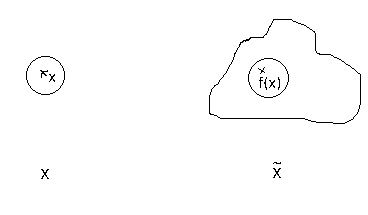
\includegraphics[scale=0.5]{fig4.png}
\end{figure}
\end{proof}
\begin{st}
Eine Abbildung zwischen metrischen Räumen ist stetig genau dann, wenn die Urbilder offener Mengen offen sind.
\end{st}
\begin{proof}
\begin{seg}{"`$\Longrightarrow$"'}
Sei $ f: X \to \tilde X $ stetig und $ V \subset \tilde Y $ offen.  Dann ist $ f^{-1}(V) $ nach \ref{st:1.8} eine Umgebung jeder ihrer Punkte somit offen.
\end{seg}
\begin{seg}{"`$\Longleftarrow$"'}
Seien umgekehrt die Urbilder offener Mengen offen und $ x \in X $. Sei $ \eps>0 $.  Nach Voraussetuuimg $ f^{-1}(B_\eps(f(x)) $ offen und enthält somit einen $ \delta $-Ball um den Punkt x.
\end{seg}
\end{proof}

Wichtige Beobachtung: Um Konvergenz und Stetigkeit zu beschreiben muss man nicht direkt auf eine Metrik Bezug nehmen, sondern es genügt das System der offenen Mengen zu kennen.  Dieses System von offenen Mengen nennt man \emph{die Topologie} des metrischen Raums .  Verschiedene Metriken können dieselbe Topologie erzeugen.

Alle Eigenschaften von metrischen Räumen, ihren Teilmengen oder Abbildung zwischen metrischen Räumen, die sich durch die Topologie (ohne direkten Bezug auf die metrik) beschreiben lassen, nennen wir \emph{topologische Eigenschaften}.

Dies führt zu dem folgenden Begriff:
\begin{df}
Sei $ X $ eine Menge und $O \in \mathcal P (x)$ eine Menge von Teilmengen von X; $ O $ heißt eine \emph{Topologie} auf $ X $, wenn folgendes gilt:
\begin{itemize}
\item[(T1)] Beliebige Vereinigungen von Mengen in $ O $ liegen wieder in O.
\item[(T2)] Die Schnittmenge von je zwei Mengen in $  O  $ liegt
\item[(T3)] Es gilt $ \emptyset \in O $ und $ X \in O$
\end{itemize}
Eine Menge $ X $ zusammen mit einer Topologie auf $ X $ heißt \emph{topologischer Raum}, die Elemente von $ O $ nennt man \emph{offene Teilmengen} von X, ihre Komplemente \emph{abgeschlossene Teilmengen}.
\end{df}
\begin{note*}
\begin{enumerate}[(\roman{enumi})]
\item Natürlich ist die Definition so gemacht, dass die in einem Topologie bilden. \fixme[fig5]
\item Verschiedene Metriken können diesselbe Topologie erzeugen, vgl. der aus der Analysis bekannter Satz, dass alle Normen auf dem $ \R^n $ äquivalent.  Daraus folgt: die Metrik die Metrik $ d(x,y) :=||x-y|| $ definiert für \emph{alle Normmen auf $ \R^n $} dieselbe Topologie, die sogenannte \emph{Standardtopologie}, zum Beispiel definieren:
\begin{align*}
d_1(x,y)&=|x_1-y_1|+...+|x_n-y_n|\\
d_2(x,y)&=\sqrt{(x_1-y_1)^2+...+(x_n-y_n)^2}\\
d_\infty(x,y)&=\max(|x_1-y_1|, ..., |x_n-y_n|)
\end{align*}
alle die Standardtopologie.
\end{enumerate}
\end{note*}
\begin{df}
Sei $ X $ ein topologischer Raum und  $x \in X $ Eine Teilmenge $ U \subset X $ heißt \emph{Umgebung} von x, wenn es eine offene Menge $ T\subset U $ gibt, die $ x $ enthält.  $ x $ heißt \emph{innerer Punkt} von A, wenn $ A $ eine Umgebung von $ x $ ist. $ x $ heißt \emph{äußerer Punkt}, falls $ X\setminus A $ eine Umgebung von x ist. Der Punkt $ x $ heißt Randpunkt von $ A $, falls keine von beiden gilt.  Die Menge $ \mathring{A} $ der inneren Punkte von $ A $ bezeichnet man als das \emph{Innere} von $ A $ oder als \emph{offener Kern} von $ A $. Die Menge $ \bar A $, der nichtäußeren Punkte von $ A $ heißt \emph{Abschluss} oder \emph{abgeschlossene Hülle} von $ A $.  Die Menge der Randpunkte von $  A $  heißt auch der Rand von A und wird mit $ \delta A $ bezeichnet. 
\end{df}

\begin{ex*}
Sei $ A=[a,b)\subset \R $ und sei $\R$ mit der Standardtopologie versuchen.  Dann gilt $\mathring A=(a,b), \bar A=[a,b], \delta A=\{a,b\}, B=\Q\subset \R$ gilt $ \mathring B=\emptyset, \bar B=\R, \delta B=\R $ 
\end{ex*}
\begin{ex}[Beispiele für Topologien]\label{thm:1.12}
\begin{enumerate}[(\roman{enumi})]
\item Durch Metriken definierte Topologie. Dies sind die sogenannten \emph{metrisierbaren Topologien}.
\item Die \emph{Klumpentopologie} $ O=\{\emptyset, X\} $ für eine beliebige Menge $ X $.  Sie ist nicht metrisierbar (falls $ X $ mehr als ein Element hat)
\item Die \emph{diskrete Topologie} $ O=\mathcal{P}(x) $ ist für jede beliebige Menge $ X $ definiert.  (Nur die schließlich konstanten Folgen sind konvergent.) Sie ist durch die diskrete Metrik gegeben.
\item Auf $\R^2$ ist durch
\[
O=\{A\subset \R^2|\forall_{(x,y)\subset A}\exists_{\eps>0}:(x-\eps,x+\eps) \times \{y\} \subset A\}
\]
eine Topologie gegeben. Übung: Ist diese metrisierbar?
\end{enumerate}

\end{ex}

\begin{df}
Sind auf einer Menge $X$ zwei Topologien $ O_1$ und $ O_2 $ gegeben, dann betrachten wir folgende Sprachweisen: gilt $ O_1 \subset O_2 $ , dann sagen wir $ O_2 $ ist \emph{feiner} als $ O_1 $ (und $ O_1 $ ist \emph{gröber} als $ O_2 $).  Gilt weder $ O_1 \subset O_2 $ noch $ O_2\subset O_1 $ , dann sagen wird, die Topologien $ O_1 $ und $ O_2 $ sind \emph{unvergleichbar}.
\end{df}

Auf jeder Menge ist die Klumpentopologie die größte mögliche Topologie und die diskrete Topologie, die feinst mögliche Topologie.  Die Topologie in \ref{thm:1.12}(iv) auf $ \R^2 $ ist feiner als die Standardtoplogie, aber gröber als die diskrete.

\begin{df}
Sei $ X $ ein topologischer Raum.  Eine Folge $ x_n $ heißt konvergent gegen $ a\in X $, falls jede Umgebung von $ a $ fast alle Folgenglieder enthält.
\end{df}
\begin{df}\label{thm:1.15}
Eine Abbildung $ f:X\to Y $ zwischen topologischen Räumen heißt \emph{stetig} in $ x\in X $, falls es zu jeder Umgebung $ V $ von $ f(x) $ eine Umgebung $ U $ von $ x $ gibt, so dass $ f(U)\subset V $ (Äquivalent: Falls das Urbild jeder Umgebung von $ x $ ist.) Die Abbildung heißt \emph{stetig}, wenn die Urbilder offener Mengen offen sind. Eine Abbildung zwischen topologischen Räumen, die bijektiv und stetig ist, heißt \emph{Homöomorphismus} (falls auch ihre Umkehrabbildung stetig ist.  Falls es einen Homöomorphismus $ d: X\to Y $ gibt, sagt man, $ X $ und $ Y $ sind \emph{homöomorph}, man schreibt: $ X\homo Y $.
Aus der Definition folgt sofort, dass eine Abbildung. $ f: X\to Y $ genau dann stetig ist, falls sie in jedem $ x\in X $ stetig ist. (zur Übung nachvollziehen)
\end{df}
\begin{st}
Sei $ f: X\to Y $ eine (in $ a\in X $) stetige Abbildung zwischen topologischen Räumen.  Sei $ x_n\to a $ konvergente Folge in $ X $. Dann gilt $ f(x_n) \to f(a) $
\end{st}
\begin{proof}
Sei $ V $ eine Umgebung von $ f(a) $. Da $ f $ (in $ a $) stetig ist, ist $ f^{-1}(V) $ eine Umgebung von $a$.  Wegen $ x_n\to a $ liegen fast alle $ x_n $ in $f^{-1}(V)$, somit gilt für fast alle $f(x_n)$ in $ V $.
\end{proof}
\begin{att}
Eine Abbildung, die jede konvergente Folge auf eine gegen das Bild des Limes konvergierende Folge abbildet (so eine Abbildung heißt \emph{folgenstetig}) ist \emph{im Allgemeinen nicht} notwendigerweise stetig. Siehe z. B. Joerich "`Topologie"' 6.3, bzw. später in der Vorlesung.
\end{att}
\begin{ex*}
\begin{enumerate}[(i)]
\item ist $ f: X\to Y $ eine stetige Abbildung und wird die Topologie auf X durch eine feinere oder die Topologie auf X durch eine gröbere ersetzt, bleibt $ f $ stetig.
\item Insbesondere ist \emph{jede} Abbildung $ f: X\to Y $ stetig falls $ Y $ die Klumpentopologie oder $ X $ die diskrete Topologie trägt.
\item In der Klumpentopologie ist \emph{jede} Folge gegen \emph{jeden Punkt} konvergent. 
\end{enumerate}
\end{ex*}
\begin{note}
Die Axiome eines topologischen Raums sind für sich alleine relativ schwach und lassen sehr viele Beispiele auch mit "`pathologischen"' Eigenschaften zu. Sie sind eher ein äußerer Begriffsrahmen. Um etwa Räume mit den von metrischen Räumen vertrauten Eigenschaften zu erhalten, muss man Zusatzannahmen machen.
\begin{itemize}
  \item "`Hausdorffeigenschaft"' $\implies$ Eindeutigkeit des Limes
  \item "`Abzählbarkeitsaxiome"' $\implies$ Äquivalenz von Stetigkeit und Folgendefinition
\end{itemize}
\end{note}
\subsection{Grundkonstruktionen}
Grundkonstruktionen sind Methoden, um neue Topologien zu definieren durch:
\begin{itemize}
\item Summe, teilräume, Produkte, Quotienten
\item durch Abbildungen zwischen topologischen Räumen
\end{itemize}
\begin{df}
Seien $ X $ und $ Y $ topologische Räume. Auf der disjunkten Vereinigung $ X \dot \cup V =X \times \{ 0 \} \cup Y \times \{1\}$ definieren wir eine Topologie durch:
\[
\{U \mathbin{\dot{\cup}} V| U \text{ offen in } X, V \text{ offen in } Y\}
\]
Der so entstehende topologische Raum $ X+Y $ wird als topologische Summe von X und Y bezeichnet (andere übliche Zeichen: $X \sqcup Y$ oder auch $X \perp Y$).
\end{df}
\begin{note*}
\begin{enumerate}[(i)]
\item Analog definert man die Summen von beliebig (auch unendlich) vieler topologischer Räumen $\biguplus_{\alpha \in  A} x_\alpha=\bigsqcup_{\alpha\in A} x_\alpha$, widerum als offene Menge $\{\dot \bigcup_{\alpha\in A}| U_\alpha \text{ offen in } X_\alpha \}$ setzt.
\item Für die disjunkte Verreinigung von Mengen $ X \dotcup Y $ ist auch die Schreibweise $X+Y:= X\times\{0\} \cup Y\times \{1\}$ üblich.  
\end{enumerate}
\end{note*}
\begin{ex*}
\begin{enumerate}[(i)]
\item Sei $ X=\{ x\} $ eine einelementige Menge. Dann ist die topologische Summe $ \biguplus_{\alpha\in A}X_\alpha $
\item Beispiel \ref{thm:1.12}(iv) ist homöomorph zu $ \biguplus_{\alpha\in \R} X_\alpha \R $ (Übung)
\end{enumerate}
\end{ex*}
\begin{df} Sei $ X $ ein topologischer Raum und $ M \subset X $. Die durch $ \{ U\cap M| U \text{ offen in } X \}$ auf $M$ defnierte Topologie heißt $ Teilraumtopologie $ (auch \emph{induzierte}, \emph{Relativ-} oder \emph{Spurtopologie}). 
\end{df}
\begin{ex*}
$X=\R^2, M=\{x-\text{Achse}\}$
\fixme[fig6]
\end{ex*}
\begin{att*}
Die offene Mengen $U\cap M$ in $ M $ sind im Allgemeinen nicht offen in $ X $ (es sei denn $ M\subset X $ wäre offen). Zum Beispiel:
\[
\text{T2: } (\underbrace{U_1}_{\text{offen in }X}\cap M)\cap (\underbrace{U_2}_{\text{offen in }X}\cap M)=(U_1\cap U_2)\cap M
\]
\end{att*}
\begin{df}
Seien $ X $ und $ Y $ topologische Räume. Eine Teilmenge $ W\subset X\times Y $ heißt offen bezüglich der Produktopologie auf $ X\times Y $ heißt offen bezüglich der Proudukttopologie auf $X\times Y$, falls es zu jedem Punkt $ (x,y)\in W $ eine Umgebung $ U $ von $ x $ und eine Umgebung $ V $ von $ y $ gibt, sodass $ U\times V $ in W enthalten ist.
\fixme[fig7]
\end{df}
\begin{note*}
\begin{enumerate}[(i)]
\item Die Standardtopologie auf $ \R^2 $ stimmt mit der Produkttopologie auf $ \R\times \R $ (beide Faktoren mit der Standardtopologie von $ \R $ versehen) überein.
\item Produkte offener Mengen in X und Y ("`Kästchen"') sind offen in den Produkttopoligien, aber nicht alle offenen Mengen sind Kästchen, z. B. sind auch die Vereinigung von Kästchen Kästchen.
\fixme[fig8] 
\end{enumerate}
\underline{Erinnerung:} Eine \emph{Äquivalenzrelation} auf einer Menge $ X $ ist eine Relation $\sim$ mit folgenden Eigenschaften:
\begin{enumerate}[(i)]
\item reflexiv: $a\sim a$
\item symmetrisch: $a\sim b \implies b\sim a$
\item transitiv: $a\sim b \land b \sim c\implies a\sim c$
\end{enumerate}
ist auf einer Menge $ X $ eine Äquivalenzrelation $\sim$ gegeben, so liegt jedes Element in seiner Äquivalenklasse
\[
 [x]:=\{y\in X|x\sim y\} \subset X
\]
und Äquivalenzklassen von zwei verschiedenen Elemente sind entweder disjunkt oder gleich; M zerfällt in die disjunkte Vereinigung der Äquivalenzklassen.  umgekehrt liefert eine Zerlegung einer Menge in disjunkte Teilmengen eine Äquivalenzrelation.
\end{note*}
\begin{df}
Sei X ein topologischer Raum und $\sim$ eine Äquivalenzrelation auf $ X $.  Sei $X/\sim$ die Menge der Äquivalenzklassen 
\[
X/\sim=\{[x]|x\in X\}
\]
und sei $ q: X\to X/\sim, x\mapsto [x] $ eine Teilmenge $ U $ von $ X/\sim $ ist genau dann offen bezüglich der \emph{Quotiententopologie} auf $ X/\sim $, wenn ihr Urbild $ q^{-1}(U) $ offen in X ist.
\end{df}

\begin{ex*}
\begin{enumerate}[(i)]
\item \begin{seg}{Zusammenschlagen eines Teilraums zu einem Punkt}
Sei $ X $ ein topologischer Raum und $ A\subset X $ ein Teilraum. Dann ist durch $ x \sim y :\equiv (x=y)\lor (x,y\in A) $ eine Äquivalenzrelation gegeben.  Zwei Punkte werden als äquivalent angesehen, wenn sie gleich sind oder beide in $ A $ liegen.
\end{seg}
\item \begin{seg}{Beispiel zu (i)}
Sei X ein topologischer Raum. Betrachte $ X\times [0,1] $
\fixme[fig9]
Man erhält den Kegel $CX:=X\times[0,1]/X\times\{1\}$
\end{seg}
\item Allgemeiner: "`\emph{Zusammenkleben}"'
\begin{enumerate}[(a)]
\item \fixme[fig10]
\item \fixme[fig11]
\end{enumerate}
bei (b) handelt es sich nicht um Zusammenschlagen eines Teilraums zu einem Punkt, sondern gegenüberliegend Punkte in den beiden senkrecht "`Radintervalle"' werden identifiziert mit den Äquivalenzrelationen: \fixme[nachschauen]
\[
(x_1,x_2)\sim (y_1,y_2):\equiv (x_1,x_2)=(y_1,y_2)\lor (x_1,y_1 \in \{0,1\} \land x_2 =y_2)
\]
\end{enumerate}
\end{ex*}
Eine weitere Möglichkeit aus gegebenen topologischen Räumen andere zu konstruieren, ist es, Topologien mit Hilfe von Abbildungen zu übertragen.
\begin{df}\label{thm:2.5}
\begin{enumerate}[(i)]
\item Sei $ X $ ein topologischer Raum und $ X $ eine Menge.  Sei $ f: X\to Y$ eine Abbildung.  Dann ist durch:
\[
\{U\subset Y|f^{-1}(U) \text{ offen} \}
\]
die \emph{finale Topologie} auf Y definiert.
\item Sei $ X $ eine Menge und $ X $ ein topologischer Raum.  Sei $ f: X\to Y $ eine Abbildung.  Dann ist durch 
\[
\{ f^{-1}(U)\subset X| U \text{ offen in } Y\}
\]
die \emph{initiale Topologie} auf X definiert.
\end{enumerate}
\end{df}
\begin{note*}
Die \emph{finale Topologie} ist die feinste Topologie auf Y die f stetig macht in (i). In (ii) ist die initiale Topologie die gröbste Topologie auf $ X $, die f stetig macht.
\end{note*}
\begin{exs*}
\begin{enumerate}[(i)]
\item Die Teilraumtopologie auf $M\subset X$ ist die initale Topologie bezüglich der \emph{Inklusionsabbildung} $ i:M\to X,m\mapsto m $, denn es gilt $ i^{-1}(U)=U\cap M $ für (offene) Mengen in $ X $.
\item Die Quotientenabbildung ist die finale Topologie bezüglich der Quotientenabbildung ist die finale Topologie bezüglich der Quotientenabbildung $ q: X\to X/\sim, x\mapsto [x] $
\item in ähnlicher Weise lässt sich die Summentopologie charakterisieren.  Sie ist die feinste Topologie, so dass beide Inklusionsabbildungen
$ i_X:X\to X+Y, x \mapsto x, i_Y: Y\to X+Y,y\mapsto y $ stetig sind.  Dies zeigt, dass es sinnvoll ist die Defnition \ref{thm:2.5} noch etwas weiter zu fassen.
\end{enumerate}
\end{exs*}
\begin{seg}{Zusatz zu Definition \ref{thm:2.5}}\label{thm:2.5(2)}
Allgemeiner definieren wir:
\begin{enumerate}[(i)]
\setcounter{enumi}{2}
\item Seien $X_i, i\in I$ topologische Räume und $ Y $ eine Menge. Sei durch $f_i:X_i\to Y, i\in I$ eine Familie von Abbildungen gegeben. Die feinste Topologie auf $ Y $, die alle Abbildungen $f_i$ stetig macht, heißt finale Topologie bezüglich $ f_i,i\in I $.
\[
\{U\subset Y|f^{-1}_i(U) \text{ offen in }X_i \text{ \emph{für alle}} i\in I\}
\]
$(T1) U_1, U_2\in O$ zeige: $U_1\cup U_2\in O$
\[f^{-1}(U_1\cup U_2)=\underbrace{f^{-1}_i(U_1)}_{\text{offen in } X_i}\cup \underbrace{f^{-1}_i(U_2)}_{\text{offen in } X_i}\]
\item Seien $ Y_i, i\in I $, topologische Räume und $ X $ eine Menge.  Seien $ f_i: X\to Y_i $ Abbildungen.  Die gröbste Topologie auf $ X $, die alle $f_i$ stetig macht, nämlich $\{f^{-1}_i\subset X| U \text{ offen in } Y, i\in I\}$ ist die \emph{initiale Topologie} bezüglich $f_i$. 
\end{enumerate}
\end{seg}
\begin{ex*}
Die Produkttopologie auf $ X\times Y $ ist initiale Topologie bezüglich der bei den kanonischen Projektionen
\[
\pi_X:X\times Y \to X, (x,y)\to x \text{ und } \pi_Y: X\times Y\to Y, (x,y)\to y 
\]
\end{ex*}
\begin{seg}{Erläuterung zu Definition \ref{thm:2.5} (iv)} 
Ist eine Familie $ S $ von offenen Teilmengen auf einer Menge $ X $ gegeben, so erhalten wir dadurch den \emph{Hüllenoperator} 
\[ 
\mathcal T(S):=\bigcap\limits_{ O \text{ Topologie auf } X \text{ mit } S\subset O} O 
\]
Die gröbste Topologie auf $ X $, die alle Mengen in $ S $ enthält. Die Topologie $ \mathcal T(S) $ nennt man auch die \emph{von $ S $ erzeugte Topologie} auf $ X $.
\end{seg}
Die in (iv) definierte Topologie ist also durch
\[
\mathcal T(\bigcup\limits_{i\in I} \{ f^{-1}(U)|U \text{ offen in } Y\} )
\]
\begin{ex}\label{thm:2.6} Sei $ \R $ mit Standardtopologie versehen. Wir definieren eine Äquivalenzklasse $ [x] $ einer reellen Zahl $ x $ ist die Menge $x+\Z=\{x+k|k\in \Z\}$. Sei $ X=R/\sim $ mit der Quotiententopologie versehen. Wir \emph{behaupten}: $ X $ ist homöomorph zu $ Y:=\{v\in \R^2|\, ||v||=1\} $, den Einheitskreis in $ \R^2 $, mit der Teilraumtopologie versehen. \fixme[fig12]
\begin{proof}
Betrachte $ \phi(t)=(\cos(2\pi\cdot t),\sin(2\pi \cdot t)), \R\to Y $.
Wegen $ \phi(t+k)=\phi(t) $ für $ k\in \Z $, ist durch $ \bar\phi: X\to Y, [x]\to \phi(x) $ eine wohldefinierte Abbildung gegeben. $\bar \phi$ ist offensichtlich bijektiv. Die Abbildung $ \bar \phi  $ ist stetig nach Definition der Quotientenabbildung, da $ \phi $ stetig ist.

Es bleibt noch zu zeigen: Die Bilder offener Mengen sind offen (man sagt dann: $ \bar \phi $ ist \emph{offen}, dass heißt die Bilder offener nicht offen), dass heißt $ \bar \phi^{-1} $ ist stetig. Wir zeigen: Die Bilder bageschlossenen Mengen sind abgeschlossen: Sei $ A\subset X $ abgeschlossen. Dann ist $ q^{-1}(A)\subset \R $ abgeschlossen (mit $ q: \R\backslash \R/\sim $ die Quotientenabbildung).

Es gilt $ \bar \phi(A)=\phi(q^{-1}(A))=\phi(q^{-1}(A)\cap[0,1]) $. Da $ q^{-1}(A)\cap [0,1] $ kompakte Tielmenge von $C$ $ \R $ ist, ist $ \bar\phi(A)=\phi(\phi-1)(A)\cap[0,1]) $ kompakt, also abgeschlossene Teilmenge des $ \R^2  $ und somit von $ Y $.
\end{proof}
\end{ex}
\subsection{Hausdorffräume}
\begin{df}[Hausdorffsches Trennungsaxiom]
 Ein topologischer Raum heißt \emph{Hausdorffraum}, wenn man zu je zwei verschiedenen Punkten disjunkte Umgebungen finden kann.
\\ \fixme[fig13]
\end{df}
\begin{st}
Jeder metrische Raum ist ein Hausdorffraum. 
\end{st}
\begin{proof}
Dies folgt aus der Dreiecksungleichung der Metrik. \\
 \fixme[fig14] \\
Seien $x$ und $y$ Punkte im metrischen Raum und sei $d(x,y)>0$.
Dann sind die beiden $\eps$-Bälle $B_\eps(x)$ und $B_\eps(y)$ mit $\eps:=\frac{1}{2}d(x,y)$ disjunkte Umgebungen von $x$ bzw. $y$. Dann 
wäre $z\in B_\eps \land B_\eps(y)$, dann wäre die Dreiecksungleichung
\[
\underbrace{d(x,z)}_{y<\eps}+\underbrace{d(z,y)}_{<\eps}\ge d(x,y)=2\eps
\]        
verletzt.
\end{proof}
\begin{st}
Jeder Teilraum eines Hausdorffraums ist Hausdorffsch. Zwei topologische Räume sind genau dann Hausdorffsch, wenn ihre topologische Summe es ist und zwei nichtleere topologische Räume sind Hausdorffsch, genau dann wenn ihr Produkt es ist. 
\end{st}
\begin{proof}[zur Übung]\end{proof}
\fixme[fig15]\\
Ein Raum, der nicht Hausdorffsch ist, scheint mit unserer Intuition unvereinbar zu sein.  Ein finales Beispiel ist die Klumpentopologie $\{\emptyset, X\}$ auf jeder Menge. Mit Hilfe der Quotiententopologie erhält man weniger triviale Beispiele von Nicht-Hausdorffräumen.
\begin{ex*} Für Nicht-Hausdorffraum:\\
Die Gerade mit einem Dppelpunkt. Sei $ X=\R+\R=\R\times \{0\}\cup \R\times \{1\} $. Definiere man $ (x,n)\sim (y,m)\stackrel{\text{def}}{\iff} x=y\neq 0 $. \\
\fixme[fig16]\\
$ \R $ besitzt unter Betrachtung dieser Relation doppelt vorhandene Nullpunkte.

Die beiden Punkte $(0,0)$ und $(0,1)$ in $ X/\sim $ lassen sich nicht durch disjunkte Umgebung trennen.\\
\fixme[fig17]\\
Wir wollen noch zwei weitere Eigenschaften von Hausdorffräumen beweisen, die mit der geometrischen Intuition übereinstimmen.
\end{ex*}
\begin{st}
In einem Hausdorffraum ist gilt:
\begin{enumerate}[(i)]
\item Der Limes einer konvergenten Folge ist eindeutig bestimmt.
\item Punkte sind abgeschlossen.
\end{enumerate}
\end{st}
\begin{proof}
\begin{enumerate}[(i)]
\item Seien $ a\neq b $ verschiedene Limiten einer konvergenten Folge $ x_n $, dann gibt es disjunkte Umgebungen $ U_a $ und $ U_b $ von $ a $ bzw. $ b $.  Da $ x_n $ gegen $ a $ konvergiert, liegen fast alle Folgenglieder in $ U_a $, im Widerspruch zur Konvergenz von $ x_n $ gegen $ b $.
\item Das Komplement einer einelementigen Menge ist offen, denn nach der Hausdorffeigenschaft gibt es um jeden ihrer Punkte eine Umgebung, die insbesondere p nicht enthält.
\end{enumerate}
\end{proof}
\fixme[fig18]
\begin{note*}
Dies liefert eine notwendige Bedingung dafür, dass eine QUotiententopologie Hausdorffsch ist.  Alle Äquivalenzklassen müssen abgeschlossen sein.
\end{note*}
\subsection{Zusammenhang und Wegzusammenhang}
\begin{df}
Ein topologischer Raum heißt \emph{zusammmenhängend}, wenn er sich nicht in zwei nichtleere, offene, disjunkte Teilmengen zerlegen lässt.
\end{df}
\fixme[fig19]
\begin{note*}
Äquivalent zu "`zusammenhängend"' sind:
\begin{enumerate}[(i)]
\item Die leere Menge und der ganze raum sind die einzigen Mengen, die sowohl offen als auch abgeschlossen sind.
\item Der Raum ist nicht homöomorph zu einer topologischen SUmme zweier nichtleere topologischer Räume.
\end{enumerate}
\end{note*}
\begin{exs*}
\begin{enumerate}[(i)]
\item Die leere Menge und der ganze Raum sind die einzigen Mengen, die sowohl offen als auch abgeschlossen sind.
\item Der Raum ist nicht homöomorph zu einer topologischen Summe zweier nichtleere topologischen Räume.
\item Ein Intervall $ I $ ist zusammenhängend: 
\begin{proof}
Angenommen $I=A\dotcup B$, beide $ A $ und $ B $ offen und abgeschlossen (in der Teilraumtopologie, durch $ I\subset \R $ induziert) Seien $ a\in A, b\in B $, wobei $ a<b $ ohne Einschränkung. Defniere $ s:=\inf\{x\in B|a<x\}$. Dann liegt in jeder Umgebung von $ s $ ein Punkt aus $ B $. (nach Definition des Infinums). Es gilt entweder $ s=a $ oder $ s>a $. Im ersten Fall kann $ s $ kein innerer Punkt von $ A $ sein, im zweiten Fall liegt das Intervall $ (a,s) $ ganz in $ A $ und $ s $ kann weder von $ A $ noch von $ B $ ein innerer Punkt sein. Dies führt letztlich zum Widerspruch.
\end{proof}
\end{enumerate}
\end{exs*}
Ein stärkerer Begriff ist der des \emph{Wegzusammenhangs} (Ein \emph{Weg} in einem topologischen Raum $ X $ ist eine stetige Abbildung $ [a,b]\to X $
\begin{df}
Ein topologischer Raum heißt \emph{wegzusammenhängend}, wenn es zu je zwei Punkte $ p,q\in X $ einen Weg gibt, dass heißt eine stetige Abbildung $ c: [0,1]\to X $ mit $c(0)=p, c(1)=q$.
\end{df}
\begin{ex*}
$ \R^n $ ist wegzusammenhängen, in der Tat, benutze man zum Beispiel $ c(t)=(1-t)p+tq $. \fixme[fig20]
\end{ex*}
\begin{st}
Ein wegzusammenhängender topologischer Raum ist zusammenhängend.
\end{st}
\begin{proof}
Angenommen $ X=A\dotcup B $, wobei $ A $ und $ B $ beide offen und nichtleer.  Sei $ p\in A $ und $ q\in B $ und $ c $ ein Weg zwischen p und q. \\ \fixme[fig21]\\
Dann wäre $[0,1]=c^{-1}(A)\dotcup c^{-1}(B)$ eine Zerlegung in zwei disjunkte, nichtleere offene Mengen.
\end{proof}
Die Umkehrung gilt jedoch im Allgemeinen nicht:
\begin{ex*}
Ein Raum, der zusammenhängend, aber nicht \underline{weg}zusammenhängend ist.
\[
X=\underbrace{\{0\}\times [-1,1]}_{A}\cup\underbrace{\{(x, \sin(x^{-1})|x>0\}}_{B}
\] 
\fixme[fig22]
\end{ex*}
Die Relation $ p\sim q \stackrel{\text{def}}{\iff} $ es gibt einen weg von $ p $ nach $ q $ ist (Übung) offensichtlich eine Äquivalenzrelation, die zugehörigen Äquivalenzklassen heißen \emph{Wegzusammenhangskomponenten} des topologischen Raums.
\begin{st}
\begin{enumerate}[(i)]
\item Stetige Bilder von (weg-)zusammenhängenden Räumen sind (weg-)zusammenhängend.
\item Vereinigungen (weg-)zusammenhängender Räume $ X_i, i\in I, $ mit $ \bigcap X_i\neq \emptyset $ sind wegzusammenhängend.
\item Ein Produkt $ X\times Y $ von (weg-)zusammenhängenden nichtleeren topologischen Räumen $ X,Y $ ist genau dann (weg-)zusammenhängend, wenn die beiden Faktoren es sind. 
\end{enumerate}
\end{st}
\begin{proof}
\item Sei $ f:X\to $ stetige Abbildung, so zerfällt $f(X)=Y_1\dotcup Y_2$ mit $Y_1, Y_2$ offen disjunkt, dann auch $ X=f^{-1}(Y_1)\dotcup f^{-1}(Y_2) $. \\
\fixme[fig23]
Sei $ p,q \in f(X) $. Es gibt $ a,b\in X $ mit $ f(a)=p $, $ f(b)=q $ und einen Weg $ c:[0,1]\to X $ von $ a $ nach $ b $. Dann ist $ f\circ c:[0,1]\to X $ ein Weg von $ p $ nach $ q $.
\item Sei $ X=\bigcup_{i\in I}X_i $. Sei $ X=A\dotcup B $ mit $ A,B $ offen. Sei $ p\in \bigcap_{i\in I}X_i $ und ohne Einschränkung $ p\in A $.  Es gilt $ X_i=(X_i\cap A)\dotcup (X_i\cap B) $, da $ p\in X_i\cap A $ folgt $ X_i\cap B=\emptyset $, denn $ X_i $ ist zusammenhängend. Also folgt $ B=\emptyset $.
Für Wegzusammenhängend:
\fixme[fig24]
Es gilt, falls $ c:[0,1]\to X_I $ estetiger Weg von $ a\in X_i $ nach $ p $ und $ d:[0,1]\to X_j $ stetiger Weg von $ p $ nach $ b\in X_j $, dann ist:
\[
e(t):=\begin{cases}c(2t)\qquad &,t\in[0,\frac 1 2]\\ d(2t-1)\qquad &,t\in[\frac 1 2, 1]\end{cases}
\]
eine stetige Abbildung $ [0,1]\to \bigcup_{i\in I}X_i $. (Übung)
\end{proof}
\begin{df}
 Eine \emph{Zusammenhangskomponente} $e$ eines topologischen Raumes $X$ ist ein maximal zusammenhängender Teilraum.
($A\subset X$ ist \emph{maximal zusammenhängend}, falls es keine zusammenhängende Teilmenge $B\subset X$ gibt mit $A\subset B, A\neq B$)
\end{df}
\begin{st}\label{thm:4.4}
 \begin{enumerate}[(i)]
  \item Ist $A\subset X$ zusammenhängend und $A\subset B\subset \bar A$, so ist auch $B$ zusammenhängend.
  \item Jeder Punkt von $X$ liegt in genau einer Zusammenghangskomponente von $X$, mit anderen Worten. $X$ ist die disjunkte Vereinigung seiner Komponenten.
\item Die Komponenten von $X$ sind abgeschlossene Teilräume.
 \end{enumerate}

\end{st}

\begin{proof}
 \begin{enumerate}[(i)]
  \item Seien $M_1,M_2\subset X$ abgeschlossen mit $B\subset M_1\cup M_2$ und $B\cap M_1\cap M_2=\emptyset$. 
Sei ohne Einschränkung $A\cap M_1\neq$. Zu zeigen ist, dass $B\cap M_2=\emptyset$. Da $A$ zusammenhängend ist, gilt $A\subset M_1$, also auch $\bar A \subset M_1$, somit gilt $B\cap M_2=\emptyset$.
\item Die Vereinigung aller zusammenhängenden Teilräume von $X$, die den Punkt $p$ enthalten, ist nach \ref{thm:4.4}(ii)
 zusammenhängend und offenbar die einzige maximal zusammenhängende Teilmenge, die $p$ enthält. (Immer ist $\{p\}$ zusammenhängend)
\item folgt aus (i).
 \end{enumerate}
\end{proof}
\subsection{Abzählbarkeitsaxiome}
\begin{df}
 Sei $(X,O)$ ein topologischer Raum. Eine Teilmenge $\mathcal B\subset O$ heißt \emph{Basis}(die Topologie) von $X$, wenn jedes $U\subset O$ eine Vereinigung von Mengen aus $\mathcal B$ ist.
\end{df}
\begin{exs*}
 \begin{enumerate}
  \item Immer gilt, dass $O$ selbst eine Basis ist.
  \item Im $\R^n$ ist der Menge der offenen $\eps$-Bälle eine Basis der Topologie, aber auch die Menge der achsenparallelen offenen Würfel.
  \item Allgemeiner ist in jedem metrischen Raum die Menge der offenen $\eps$-Bälle eine Basis der Topologie.
  \item Seien $(X_1,O_2)$ und $(X_2,O_2)$ topologische Räume. Dann ist $O_1\times O_2$ eine Basis der Produkttopologie.
\end{enumerate}
\end{exs*}
Kann man beliebige Familien von Teilmengen eines Raumes $X$ vorgeben und fordern, die Topologie solle aus allen Vereinigungen dieser Mengen (und $X$ selbst) bestehen? Nein, man muss auch sicherstellen, dass endliche Schnitte wieder offen sind. Deshalb:
\begin{df}
 Sei $(X,O)$ ein topologischer Raum. Eine Teilmenge $\mathcal S\subset O$ heißt \emph{Subbasis}, wenn die Menge der endlichen Schnitte der Mengen in $\mathcal S$ eine Basis bildet.
\end{df}
\begin{st}\label{thm:4.3}
 Sei $X$ eine Menge und $\mathcal S\subset \Pot(X)$  eine Familie von Teilmengen von $X$. Dann gibt es genau eine Topologie auf $X$, die dieses $S$ als Subbasis hat.
\end{st}
\begin{proof}
Sei $\mathcal B:=\{S_1\cap...\cap S_n|n\in \N_0, S_1,...,S_n\in \mathcal S\}$ und setze $O:=\{\bigcup_iB_i|i\in \mathcal B\} \cup\{\emptyset,X\}$.
 Wir zeigen, dass $O$ eine Topologie auf $X$ ist. Offensichtlich liegen beliebigen Vereinigung von Mengen in $O$ wieder in $O$. 
Sei $U_1=\bigcup_{i\in I_1}B_i, U_2=\bigcup_{i\in I_2}B_i$, mit $B_i\in \mathcal B$. Dann ist:
\[
 U_1\cap U_2=\bigcup\limits_{j\in I_1,k\in I_2}B_j\cap B_k
\]
eine Vereinigung von endlichen Schritten von Mengen in $\mathcal S$, also Element von $O$. (Dies zeigt, dass $O$ eine Topologie auf $X$ ist). 
Jede Topologie auf $X$, die $\mathcal S$ enthält, muss auch $O$ enthalten, anderer seits kam eine Topologie mit $\mathcal S$ als Subbasis auch nicht feiner sei als $O$.
\end{proof}
Man sagt auch, $O$ ist die \emph{von $\mathcal S$ erzeugte Topologie}. Dass heißt $O$ entsteht durch Anwenden des früher definierten
Hüllenoperators auf $\mathcal S$, $\mathcal T(\mathcal S)=\emptyset$.

Als eine Anwendung wollen wir die Produkttopologie von beliebig (auch unendlich) vielen Räumen erklären.

Seien $(X_\alpha,O_\alpha), \alpha A$ topologische Räume und sei
\[
 \bigsqcap X_\alpha=\{f:A\to\bigcup X_\alpha|f(\alpha)\in X_\alpha\}
\]
Wir verwenden als Subbasis die Menge
\[
 \mathcal S:=\{\bigsqcap_\alpha U_\alpha\in O_\alpha, U_\alpha=X_\alpha \text{ für alle bis auf ein $\alpha \in A$}\}
\]
Die so (nach Satz \ref{thm:4.3}) defnierte Topologie heißt \emph{Produkttopologie} auf $\bigsqcap_\alpha X_\alpha$ (und 
$\mathcal S$ ist eine Subbasis). Dann ist:
\[
 \mathcal B := \{ \bigsqcap_\alpha U_\alpha|U_\alpha\in O_\alpha, U_\alpha=X_\alpha \text{ für alle bis auf endlich viele } \alpha \in A\}
\]
\begin{seg}{Übungsaufgabe}
 Nach Konstruktion ist die Produkttopologie die initiale Topologie bezüglich der kanonischen Projektionen $\pi_\alpha:\bigsqcap_\alpha X_\alpha\to X_\alpha: f\mapsto f(\alpha)$
Die kanonische Projektionenen sind nämlich stetig: Sei $\alpha \in A$. Das Urbild $\pi_\alpha^{-1}$ einer offenen Menge $U\subset X_\alpha$ ist gerade:
\[
 \{\bigsqcap_\beta U_\beta|U_\alpha=U, U_\beta=X_\beta \text{ für } \beta\neq a\}
\]

\end{seg}
\begin{note*}
 \begin{itemize}
  \item $\mathcal S=(X_1,X_2,...,X_{k-1}, U, X_{k+1},...,X_n$ mit $U\subset X_k$ offen,$A={1,...,n}$
  \item $\R^3=\{(x_1,x_2,x_3)|x_\alpha\in \R\}$, $\R^3=\{f:\{1,2,3\}\mapsto \R, \alpha\mapsto x_\alpha\}$
 \end{itemize}
\end{note*}
\begin{df}
 Sei $(X,O)$ ein topologischer Raum. Eine Familie $\mathcal U$ von Umgebungen von $p$ heißt \emph{Umgebungsbasis} von $p$, wenn jede Umgebung von $p$ eine Umgebung aus U enthält.
\fixme[fig25]
\end{df}
\begin{exs*}
 \begin{enumerate}
\item  Im $\R^n$ ist zum Beispiel ist $
 \{B_\eps(p)|\eps>0\}$ eine Umgebungsbasis von $p$, aber auch $ \{B_\eps(p)|\eps\in (0,1]\}$ und $\{ B_\eps(p)|\eps>0,\eps\in \Q \}$ die letzte ist abzählbar auch $\{B_{n^{-1}}(p)|n\in \N\}$
\item Dies lässt sich auf metrische Räume übertragen: In jedem metrischen Raum $X$ mit $p\in X$ ist $\{B_{n^{-1}}(p)|n\in \N\}$ eine abzählbare Umgebungsbasis von p.
 \end{enumerate}
\begin{df}
 \begin{enumerate}[(i)]
  \item Ein topologischer Raum erfüllt das \emph{erste Abzählbarkeitsaxiome}, wenn es um jeden Punkt eine abzählbare Umgebungsbasis gibt. 
\item Ein topologischer Raum erfüllt das \emph{zweite Abzählbarkeitsaxiome}, wenn es eine abzählbare Basis der Topologie gibt.
 \end{enumerate}

\end{df}
\end{exs*}
\begin{seg}{Zusammenfassung}
\begin{itemize}
 \item \emph{Basis}, wenn sich jede offene Teilmengen als Vereinigung dieser Menge bilden lässt.
 \item \emph{Subbasis}, wenn endliche Schnitte eine Basis bilden.
 \item \emph{Abzählbarkeitsaxiome}
 \begin{itemize}
\item \emph{Erstes Abzählbarkeitsaxiom}: Um jeden Punkt gibt es ein abzählbare \emph{Umgebungsbasis}(Umgebungsbasis von $p\in X$: eine Familie von Teilmengen $U$
, wenn jede Umgebung von p eine Menge aus $U$ enthält.)
\item \emph{Zweites Abzählbarkeitsaxiom}: Der Raum besitzt eine abzählbare Basis
\end{itemize}
\end{itemize}
\end{seg}
Der folgende Satz gibt eine Antwort auf die Frage, wie die beiden Abzählbarkeitsaxiome zusammenhängen und eine Antwort auf die Frage, wozu das erste Abzählbarkeitsaxiom nützlich ist.
\begin{st}\label{thm:5.6}
 \begin{enumerate}[(i)]
  \item Das zweite Abzählbarkeitsaxiom impliziert das erste.
  \item Gilt in einem topologischen Raum $X$ das erste Abzählbarkeitsaxiom, dann sind Stetigkeit und Folgenstetigkeit für Abbildungen $f:X\to X$ äquivalent.
 \end{enumerate}
\end{st}
\begin{proof}
 \begin{enumerate}[(i)]
  \item Sei $\mathcal B$ eine abzählbare Basis der Topologie und $p\in X$ ein beliebiger Punkt. Setze $\mathcal U:=\{U\in \mathcal{B} |p\in U\}$. Sei nun $V$ eine Umgebung von $p$, dann enthält eine offene Menge $Q$ mit $p\in Q$. Aber $Q$ ist eine Vereinigung von Mengen in $\mathcal B$, also gibt es eine Menge $U\in \mathcal B$ mit $p\in U$, für diese gilt $U\in \mathcal U$.
\item \begin{seg}{„$\implies$“} bereits gezeigt in \ref{thm:1.15} \end{seg}
\begin{seg}{„$\implies$“} Sei nun $f:X\to Y$ folgenstetig und gelte in $X$ das erste Abzählbarkeitsaxiom. Angenommen, f wäre \emph{nicht} stetig in einem Punkt $x\in X$. Dann gibt es eine Umgebung $U$ von $f(x)$, zu der es \emph{keine} Umgebung $V$ von $x$ gibt mit $f(V)\subset U$.
 Sei $\mathcal U=\{U_1,U_2,U_3,...\}$ eine abzählbare Umgebungsbasis von $x$. 
Die Mengen $U_1, U_1\cap U_2$, $U_1\cap U_2,\cap U_3,...$ Umgebungen von $x$. 
Nach Annahme gibt es in jeder dieser Mengen $U_1\cap...\cap U_k$ einen Punkt $x_n$, so dass $f(x_n)$ außerhalb 
von U liegt. Die Folge $x_n$ konvergiert gegen $x$, die Folge $f(x_n)$ aber \emph{nicht} gegen f(x).
\end{seg}
\end{enumerate}
\end{proof}
\begin{note}
 $f: X\to Y$ heißt \emph{folgenstetig}, falls für alle konvergenten Folgen $x_n\to x$ in $X$ gilt $f(x_n)\to f(x)$.von 
\end{note}
\subsection{Kompaktheit}
\begin{df}\label{thm:6.1}
 Eine \emph{offene Überdeckung} eines topologischen Raumes $X$ ist eine Familie $U_i$, $i\in I$, von offenen Teilmengen von $X$ mit der Eigenschaft $\bigcup_{i\in I} U_i=X$.
\end{df}
\begin{df}\label{thm:6.2}
 Ein topologischer Raum $X$ heißt \emph{kompakt}, wenn jede offene Überdeckung von $X$ heißt \emph{kompakt}, wenn jede offene Überdeckung von $X$ eine \emph{endliche Teilüberdeckung} besitzt, dass heißt falls folgendes gilt: ist $U_i, i\in I$, eine offene Überdeckung von $X$, so gibt es endlich viele $i_1, ...,i_n\in I$, so dass $U_{i_1}\cup ...\cup U_{i_n}=X$ gilt.
\end{df}
\begin{ex*}
 $\R^n$ ist \emph{nicht kompakt}, denn die offene Überdeckung durch $B_k(0),k\in \N$ besitzt eine endliche Teilüberdeckung.
\end{ex*}

\begin{note}\label{thm:6.3}
 Manchmal (nicht in dieser Vorlesung) wird zusätzlich noch die Hausdorffeigenschaft verlangt (in diesem Fall heißt die obige Eigenschaft meist "`präkompakt"').
\end{note}
\begin{st}[Heine-Borelscher Überdeckungssatz]\label{thm:6.4}
 Eine Teilmenge des $\R^n$ ist kompakt genau dann, wenn sie abgeschlossen und beschränkt ist.
\end{st}
\begin{proof}
 siehe zum Beispiel Forster O., Analysis II.
\end{proof}
\begin{st}\label{thm:6.5}
 Jede kompakte Teilmenge eines metrischen Raumes ist beschränkt und abgeschlossen (Umkehrung gilt im Allgemeinen nicht).
\end{st}
\begin{proof}
 \begin{seg}{Beschränktheit}
  Für einen beliebigen Punkt $x$ bildet $B_k(x)\cap A, k \in \N$, eine offene Überdeckung von $A$, da es eine endliche Teilüberdeckung gibt, 
ist der Abstand von x durch eine natürliche Zahl beschränkt.
 \end{seg}
\begin{seg}{Abgeschlossen}
 Sei $A\subset X$ kompakt und sei $x\in X\setminus A$. Es gilt:
\[
 U_\eps:=(X\setminus\bar{B_\eps(x)})\cap A, \eps>0 := \{ y\in X|d(x,y)\le \eps\}
\]
bilden eine offene Überdeckung von $A$, es gibt eine endliche Teilüberdeckung $U_{\eps_1}\cup... \cup U_{\eps_k}$, und es folgt, dass $B_\eps(x)$ mit $\eps:=\min\{\eps_1,...,\eps_k\}$ ganz in $X\setminus A$ liegt.

\fixme[fig26]
\end{seg}
\end{proof}
Die Umkehrung gilt in beliebigen metrischen Räumen \emph{nicht}, der Begriff „beschränkt“ lässt sich nicht analog auf metrische Räume übertragen, denn für jede Metrik $d$ auf $X$ ist auch
\[
 d'(x,y):=\frac{d(x,y)}{1+d(x,y)}<1
\]
eine Metrik (die dieselbe Topologie erzeugt) also ist die Unterscheidung zwischen beschränkten und unbeschränkten Mengen hier nicht sehr hilfreich.
\begin{note*}
 Ein metrischer Raum ist kompakt, wenn er \emph{vollständig} und \emph{totalbeschränkt} ist, \emph{totalbeschränkt} bedeutet: zu jedem $\eps>0$ gibt es ein endliches $\eps$-Netz, dass heißt zu jedem $\eps>0$ gibt es endlich viele Punkte $x_1,...,x_k$ mit $\bigcup_{i=1}^kB_\eps(x_i)=X$.
\end{note*}
\begin{st}\label{thm:6.6}
 Stetige Bilder kompakter Räume sind kompakt
\end{st}
\begin{proof}
Sei $f:X\to Y$ stetig und $U_i, i\in I$ eine offene Überdeckung von $Y$. Dann ist $f^{-1}(U_i),i\in I$, eine offene Überdeckung von $X$. Diese besitzt aber eine endliche Teilüberdeckung $f^{-1}(U_i)\cup ...\cup f^{-1}(U_{i_n})=X$. Dann ist $U_{i_1}\cup ...\cup U_{i_n}$ eine offene Überdeckung von $Y$, falls $f$ surjektiv ist.
\end{proof}
\begin{st*}
 Abgeschlossene Teilräume von kompakten Mengen sind kompakt.
\end{st*}
\begin{proof}
 Sei $X$ kompakt, $A\subset X$ abgeschlossen. Sei $U_i, i\in I,$ eine offene Überdeckung von $A$.
\begin{figure}[h]
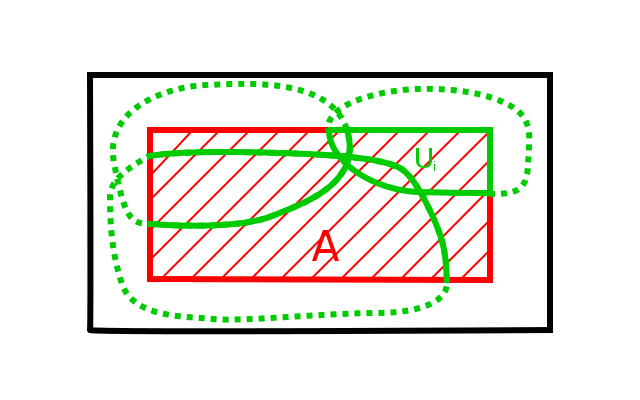
\includegraphics[scale=0.5]{fig27.png}
\end{figure}

\fixme[Grafik stimmt nicht überein]\\

Nach Definition der Teilraumtopologie gibt es offene Mengen $V_i$ von $X$, so dass $U_i=V_i\cap A$. Dann ist 
\[
 (X\setminus A) \cup \bigcup_{i\in I} V_i
\]
eine offene Überdeckung von $X$, diese hat eine endliche Teilüberdeckung der Form 
\[
(X\setminus A)\cup V_{i_1} \cup...\cup V_{i_n}
\]
Somit überdecken die Mengen $U_{i_1}=V_{i_1}\cap A, ..., U_{i_n}=V_{i_n}\cap A$ ganz $A$.
\end{proof}
\begin{st} \label{thm:6.7}
In einem Hausdorffraum sind kompakte Teilräume abgeschlossen.
\end{st}
\begin{proof}
 Sei $X$ ein Hausdorffraum und $A\subset X$ kompakt mit der induzierten Topologie. Wir wollen zeigen, dass es um jeden Punkt $x\in X\setminus A$ eine Umgebung gibt, die A nicht trifft, dann ist $X\setminus A$ offen. Sei $p\in X\setminus A$. Nach der Hausdorffeigenschaft von $X$ finden wir zu jedem $a\in A$ eine Umgebung $U_a$ von $a$ und eine Umgebung $V_a$ von $p$, so dass $U_a\cap V_a=\emptyset$ für \\
\begin{figure}[h]
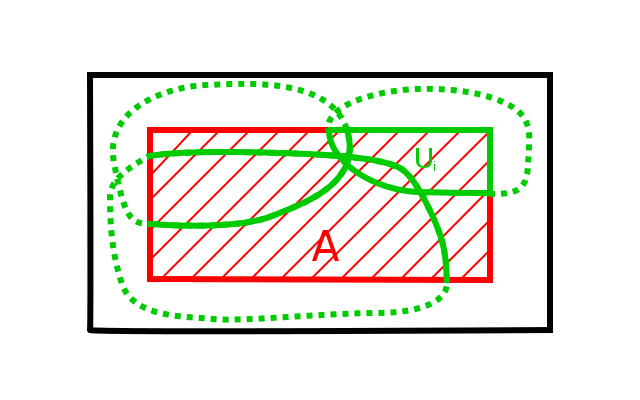
\includegraphics[scale=0.5]{fig28.png}
\end{figure}
<<<<<<< HEAD
\fixme[passt nicht]
=======
\fixme[Grafik stimmt nicht überein]\\
>>>>>>> 0b3fb6935622bc43c6a1dffd8416eaad76deee9e
alle $a\in A$ Der Schnitt aller $V_a, a\in A$ ist möglicherweise nicht offen (da eventuell Schnittmenge unedlich vieler Mengen.
$U_{a_1},..., U_{a_n}$ auswählen, so dass $A\subset U_{a_1}\cup...\cup U_{a_n}$. Dann gilt: $V_{a_1}\cap...\cap V_{a_n}$ ist offen und liegt ganz im Komplement von $A$.
\end{proof}
Insgesamt folgt aus Satz \ref{thm:6.6} und Satz \ref{thm:6.7}, dass in einem kompakten Hausdorffraum \underline{die} Abgeschlossenheit und Kompaktheit von Teilräumen äquivalent sind.
\begin{st}\label{thm:6.8}
 Sei $X$ ein kompakter topologischer Raum und $Y$ ein Hausdorffraum. Sei $f: X\to Y$ eine stetige bijektive Abbildung. Dann ist $f$ ein Homöomorphismus
\end{st}
\begin{proof}
 Es ist nur zu zeigen, dass $f$ die Eigenschaft hat, dass Bilder offener Mengen offen sind (dann sind die Urbilder offenen Mengen unten der Umkehrabbildung $f^{-1}:Y\to X$ offen)

Äquivalent dazu: Die Bilder abgeschlossener Mengen sind abgeschlossen. Sei $A\subset X$ abgeschlossen, da $X$ kompakt, ist A nach 6.6 auch kompakt, also ist $f(A)$ ein kompakter Teilraum von $Y$. Da $Y$ Hausdorffsch folgt aus \ref{thm:6.7}, dass $f(A)$ abgeschlossen ist.
\end{proof}
\begin{ex*}
 \begin{enumerate}[(i)]
  \item Sei $X=\R/\sim$ wie im Beispiel \ref{thm:2.6}, $x\sim y:\iff x-y\in \Z$ und sei $Y=S^1$ (der Einheitskreis in $\R^2$). Dann ist $X=\R/\sim$ kompakt nach \ref{thm:6.5}, da Bild der kompakten Teilmenge $[0,1]$ von $\R$. Andererseits ist $Y$ offensichtlich als Teilraum des Hausdorffraums $\R^2$ ebenfalls Hausdorffsch.
Die Abbildung $\phi: \R\to Y, t\to e^{i2\pi t}$ (bzw. $(\cos(2\pi t), \sin(2\pi t))^T$) ist stetig, also auch $\bar \phi: \R/\sim \to Y, [t]\to e^{i2\pi t}$, da $\bar \phi$ bijektiv ist, folgt, daraus $\bar \phi$ ein Homöomorphismus ist, insbesondere gilt $\R/\sim \homo S^1$

 \item $S^1=\{(x,y)^T\in \R^2|x^2+y^2=1\}=\{z\in \C||z|=1\}$\\
\begin{figure}[h]
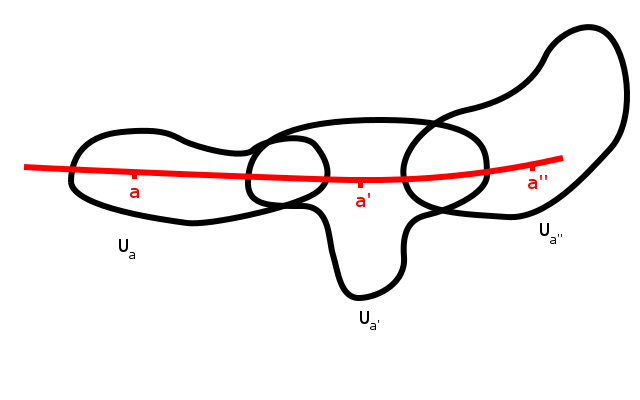
\includegraphics[scale=0.5]{fig29.png}
\end{figure}
<<<<<<< HEAD
\fixme[passt nicht]
=======
\fixme[Grafik stimmt nicht überein]
>>>>>>> 0b3fb6935622bc43c6a1dffd8416eaad76deee9e
 Sei $X:=S^1/\sim$ $z\sim z':\iff z=z'$ oder $z=-z'$ $X$ ist kompakt, da Bild des kompakten EInheitskreises $S^1$ unter der Quotientenabbildung. WIr wollen zeigen, dass $X\homo S^{1}$ gilt. Definiere $f:X\to S^1$ durch $[z]\to z^2$. Dann ist $f$ wohldefiniert, bijektiv und stetig i
ist, ($q$ ist die Quotientenabbildung). Nach \ref{thm:6.8} folgt $X\homo S^1$ (bzw. $\R P^1\homo S^1$)

Wie bei der Stetigkeit kann man Kompaktheit auch (in gewissen Räumen) durch Folgen beschreiben
\end{enumerate}
\end{ex*}
\begin{df}\label{thm:6.9}
 Ein topologischer Raum heißt \emph{folgenkompakt}, wenn jede Folge eine konvergente Teilforge besitzt.  
\end{df}
\begin{ex*}
 Folge $x_n, n\in \N$ Teilfolge $x_{n_k}$ mit $k\to n_k$ steigt monoton steigend. zum Beispiel hat $a_n=(-1)^n+\frac 1 n$ die konvergente Teilfolgen $a_{2n}$ und $a_{2n+1}$
\end{ex*}
\begin{st}\label{thm:6.10}
 In topologischen Räumen, die das zweite Abzählbarkeitsaxiom erfüllen (dass heißt es gibt eine abzählbare Basis der Topologie) sind Folgenkompaktheit und \emph{Überdeckungskompaktheit} (dass heißt Kompaktheit wie in \ref{thm:6.2} defniert) äquivalent.
\end{st}
Zum Beweis benötigen wir zwei Lemmata.
\begin{lem}\label{thm:6.11}
 Sei $x_n, n\in \N$, eine Folge in dem topologischen Raum $X$, der das erste Abzählbarkeitsaxiom erfüllt.  Dann gilt: $x_n$ besitzt genau darin eine konvergente Teilfolge, wenn ein $x\in X$ existiert, so dass in jedem Umgebung $U$ von $x$ unendlich viele Folgenglieder $x_n$ in $U$ liegen.
\end{lem}
\begin{proof}
 \begin{seg}{"`$\implies$"'}
  Gelt $x_{n_k}\to x$ und sei $U$ Umgebung von $x$, dann gibt es $k_0\in \N$, so dass $X_{n_k}\in U$ für $k\ge k_0$.
 \end{seg}
\begin{seg}{"`$\Longleftarrow$"'}
 Sei umgekehrt die obige Bedingung erfüllt und $U_1\supset U_2 \supset ...$ eine Umgebungsbasis von $x$. Wir wählen
$x_{n_1}\in U_1, x_{n_2}\in U_2$ mit $n_1<n_2<...<n_k<...$. Die letzte Bedingung erfüllbar, da im Inneren unendlich viele Indies $n$ mit $x_n\in U_k$ existieren. Damit ist $x_n\to x$ offensichtlich.
\end{seg}
\end{proof}
 Wir haben bereits gezeigt in Lemma \ref{thm:6.11}. Sei $x_n$ eine Folge in den topologischen Raum  mit abzählbaren Umgebungsbasis. Dann gilt: $x_n$ besitzt genau dann eine onvergente Teilfolge , wenn ein $x\in X$ existiert, so dass 
in jeder Umgebung $U$ von $x$ unendlich viele Folgenglieder liegen. Wir wollen nun \ref{thm:6.10} beweisen. Dafür benötigen wir noch ein Lemma.
\begin{lem}\label{thm:6.12}
 Erfüllt $X$ das zweite Abzählbarkeitsaxiom,  so enthält jede offene Überdeckung eine abzählbare Teilüberdeckung
\end{lem}
\begin{proof}
 Sei $O_1,O_2,...$ eine abzählbare Basis der TOpologie. Sei $X=\bigcup_{\alpha\in A} U_\alpha$, $U_\alpha$ 
offen (wir wollen zeigen:  es gibt $a_1, a_2,...,$ so dass $X=\bigcup_{\alpha\in A}U_\alpha$). 
Setze $\N'=\{n\in \N|O_\alpha\in U_\alpha \text{ für ein } A\}$.
Für $n\in \N'$ wählen wir $\alpha_n\in A$ mit $O_n\subset U_{\alpha_n}$. Dann ist $\{U_{\alpha_n}\}_{n\in \N'}$ eine (abzählbare) Überdeckung von $X$. 
Denn jedes $x$ liegt in einem $U_\alpha$. Da die $\alpha_n$ eine Basis bilden ist $U_\alpha$ eine Vereinigung von solchen, also existiert ein $n$ mit $x\in O_n\subset U\alpha$, insbesondere $n\in \N'$ und $x\in U_{\alpha_n}$ .
\end{proof}
\begin{seg}{\textbf{Beweis von Satz \ref{thm:6.10}}}
 Sei $X$ ein Raum mit abzählbarer Basis.
\begin{enumerate}[(i)]
 \item Sei $X$ kompakt und $x_n$ eine Folge ohne konvergente Teilfolge. Nach \ref{thm:6.11} gibt es zu jedem $p\in X$ eine Umgebung $U_p$ mit $x_n\in U_p$ nur für endlich viele Indizes $n$. Die $U_p$ bilden eine Überdeckung. Wegen der Kompaktheit gibt es ensgesamt ist $x_n\in U_{p_1}\cup... U_{p_k}=X$ nur für endlich viele Indizes. Dies ergibt den Widerspruch.
 \item Sei $X$ folgenkompakt und eine offene Überdeckung vorgegeben. Nach \ref{thm:6.12} enthält sie eine abzählbare Teilüberdeckung, etwa $U_1, U_2, ...$ Können wir aus dieser keine endliche Teilüberdeckung auswählen, dann gilt $X\neq \bigcup_{k=1}^nU_k$ für ale $n$, dass heißt es gibt $x_n\in X\setminus(U_1\cup...\cup U_n)$. Wegen Folgenkompaktheit hat $x_n$ eine konvergente Teilfolge $x_n \to x$ und $x\in U_m$ für ein $m\in \N$. Dann gilt $x_{n_k}\in U_m$ für alle $k$ ab einer Schranke. Dies ergibt den Widerspruch.
\end{enumerate}
\end{seg}
\begin{note*}
 \begin{enumerate}[(i)]
  \item Für die Richtung „kompakt $\implies$ folgenkompakt“ benötigen wir nur das erste Abzählbarkeitsaxiom. 
Insbesondere gilt die Aussage in metrischen Räume.  
(Dies impliziert die Beschränktheit kompakter metrischer Räume und ihre Teilmengen Hausdorff, folgt nochmal \ref{thm:6.4})
\item Auch Satz \ref{thm:6.3} (Heine-Borel) folgt aus dem letzten Satz: Ist $A\subset \R^n$ beschränkt und abgeschlossen, so besitzt jede Folge nach Bolzano eine konvergente Teilfolge.
Also ist $A$ folgenkompakt. Da $\R^n$ (und damit $A$) eine abzählbare Basis (nämlich zum Beispiel $\{B_{n^{-1}} (q)|n\in \N, q\in \Q^n\}$ besitzt,
ist $A$ kompakt. Die andere Richtung folgt aus Bemerkung (i).
\item In einem Banachraum ist die Einheitskugel genau dann kompakt, wenn die Dimension endlich ist,
\item Andererseits: Satz von Tychonoff: Beliebige Produkte kompakter Räume sind kompakt.
 \end{enumerate}
\end{note*}
\subsection{Topologische Mannigfaltigkeiten}
\begin{df}[$n-$dimensionale eingebettete Untermannigfaltigkeit des $\R^{n+k}$]
Eine Teilmenge $M\subset \R^{n+k}$ heißt \emph{$k$-dimensionale Untermannigfaltigkeit} des $\R^{n+k}$, falls es um jeden Punkt $p\in M$ eine (im $\R^{n+k}$) offene Menge, $U$ gibt und einen Diffeomorphismus $\Phi: U\to V$, wobei $V\subset \R^{n+k}$ offen ist und gilt:
\fixme[fig30]
\[
 \boxed{\Phi(U\cap M)=V\cap(\R^n\times(\underbrace{0,...,0}_{k-\text{mal}}))}
\]
\end{df}
\begin{exs*}
 \begin{enumerate}[(i)]
  \item offene Mengen im $\R^n$ sind $n-$dimensionale Untermannigfaltigkeit.
  \item lineare (affine) Unterräume (Punkte, Geraden, Ebenen,...) sind Untermannigfaltigkeiten
  \item Die Einheitsphäre $S^n\subset \R^{n+1}$ ist eine $n-$dimensionale Untermannigfaltigkeit
  \item Dass (iii) gilt, zeigt man zum Beispiel, indem man nachrechnet, dass $S^n$ ein \emph{reguläres Urbild} ist. Zum Beispiel ist $S^n$ das Urbild $f^{-1}(\{1\})$ der Abbildung $\R^{n+1}\to \R, (x_1,...,x_n+1)\mapsto x_1^2+...+x_{n+1}^2$
 \end{enumerate}
Mannigfaltigkeiten sind Räume, die im Kleinen den Euklidischen Raum $\R^n$ ähneln, aber nicht notwendig im Großen.
\end{exs*}
\begin{df}
 Ein topologischer Raum heißt \emph{n-dimensionale topologische Mannigfaltigkeit}, wenn $M$ Hausdorffsch ist, eine abzählbare Basis hat und lokal homöomorph zum $\R^n$ ist, dass heißt für alle $p\in M$ existiert ein Homöomorphismus $\phi:U\to V$, wobei $U$ offene Umgebung von $p$ in $M$ ist und $V$ offen im $\R^n$.
\end{df}orffsch ist, eine abzählbare Basis hat und lokal homöomorph zum $\R^n$ ist, dass heißt für alle $p\in M$ existiert ein Homöomorphismus $\phi:U\to V$, wobei $U$ offene Umgebung von $p$ in $M$ ist und $V$ offen im $\R^n$.
\fixme[fig31]
\begin{note*}
 \begin{enumerate}[(i)]
  \item $n-$dimensionale Untermannigfaltigkeit der $\R^{n+k}$ sind $n$-dimensionale topologische Mannigfaltigkeit
  \item Indem wir $\phi$ eventuell einschränken, können wir für $V$ einen offenen Ball nehmen, oder wir können $V$ als $\R^n$ wählen (da offene Bälle im $\R^n$ homöomorph zu $\R^n$ sind, Übungsaufgabe)
  \item Muss lokal aussehen wie $\R^n$. Keine topologische Mannigfaltigkeit sind.\\
\fixme[fig32]\\
\item Im Gegensatz zu Untermannigfaltigkeit hat man keine „Glattheitsbedingung“ so ist zum Beispiel ein Quadrat im $\R^2$ eine topologische Mannigfaltigkeit.
 \end{enumerate}
\end{note*}
Es gilt: Die Summe zweier n-dimensionale topologische Mannigfaltigkeit ist wieder eine $n$-dimensionale topologische Mannigfaltigkeit. Das Produkt einer $n-$dimensionalen und einer $m$-dimensionaler topologischen Mannigfaltigkeit ist eine $(n+m)$-dimensionale topologische Mannigfaltigkeit. Das Produkt einer n-dimensionaler topologischen Mannigfaltigkeit ist eine $(n+m)-$dimensionale topologische Mannigfaltigkeit. Offene Teilmengen von $n-$dimensionale toppologische Mannigfaltigkeit sind $n$-dimensionale topologische Mannigfaltigkeit. Für Quotienten von topologischen Mannigfaltigkeit ist die Frage, ob sie wieder topologische Mannigfaltigkeiten sind, kompliziert.
Zum Beispiel Gerade mit Doppelpunkt\\
\fixme[fig33]\\
Ein Summe in zwei $n$-dimensionale topologischen Mannigfaltigkeiten ist wieder eine $n$-dimensionale topologische Mannigfaltigeit, das Produkt einer $n$-dimensionalen Mannigfaltigkeit mit einer $m$-dimensionalen Mannigfaltigkeit ist eine $(n+ m)$-dimensionale topologische Mannigfaltigkeit und außerdem sind offene Teilmengen von $n$-dimensionale topologische Mannigfaltigkeiten wieder $n$-dimensionale topologische Mannigfaltigkeiten.  

Die Konstruktion vom Quotient dagegen ist delikater. Wir begnügen uns mit einem einfachen Fall.

Die Homöomorphismen eines topologischen Raumes $\{\phi: X\to X|\phi \text{ Homöomorphismus}\}$ bilden eine Gruppe, denn die Hintereinanderschaltung von Homöomorphismen ist wieder einer, die Umkehrabbildung eines Homöomorphismus liefert das Inverse, die Identität das neutrale Element.

Wir betrachten (endliche) Untergruppen $\Gamma$ von Homöomorphismen, zum Beispiel $X=S^n, \Gamma=\{\pm \id\}$ , wobei $\id: S^n\to S^n$ die Antipodenabbildung $x\mapsto -x$ ist. Ist $\Gamma$ eine Gruppe von Homöomorphismen auf $X$, so setzen wir $X/\Gamma:=X/\sim$, wobei die Äquivalenzrelation $\sim$ auf $X$ wie folgt gegeben ist.
\[
 x\sim y :\iff \text{ es gibt ein } \gamma\in \Gamma \text{ mit } y=\underbrace{\gamma(x)}_{:=\gamma(x)}
\]
\begin{itemize}
\item \emph{reflexiv}, dass heißt $x\sim x$, da $\id_X\in \Gamma$
\item \emph{symmetrisch}, dass heißt $x\sim y \implies y\sim x$, denn fals $y=\gamma(x)$, dann folgt $x=\gamma^{-1}(y)$
\item \emph{transitiv}, dass heißt $x\sim y \land y\sim z \implies x\sim z$, denn $y=\gamma(x), z=\gamma'(y)$, dann folgt $\gamma'\circ \gamma(x)=\gamma'\circ y=z$, also $(\gamma'\circ \gamma)(x=y)$. 
\end{itemize}
Dann sind die Äquivalenzklassen die \emph{Bahnen} der Operation der Operation von $\Gamma$ auf $X$, wobei die \emph{Bahn} des Punktes $x$ die Menge $\Gamma x:=\{\gamma(y)$ ist.

Zum Beispiel falls $X=S^n, \Gamma=\{\pm \id\}$, dann ist $\Gamma x=\{\pm x\}$. Wir versehen $X/\Gamma$ mit der Quotiententopologie. Gilt für $\gamma:X\to X$ und einen Punkt $x\in X$, dass $\gamma(x)=x$, dann nennt $\max(x)$ einen \emph{Fixpunkt} von $\gamma$. Die Identität hat natürlich jeden Punkt als Fixpunkt.
\begin{df}
 Eine Gruppe $\Gamma$ von Homöomorphismen operiert \emph{fixpunktfrei} auf $X$, wenn nur die Identität Fixpunkte auf $x$ hat, dass heißt falls aus $\gamma x=x$ für ein $\gamma\in \Gamma$ folgt, dass $\gamma=\id_x$.
\end{df}
\begin{st}\label{thm:7.4}
 Sei $M$ eine $n$-dimensionale topologische Mannigfaltigkeit und $\Gamma$ eine endliche Gruppe von Homöomorphismen, 
die fixpunktfrei auf $M$ operiert. Dann ist $M/\Gamma$ eine $n$-dimensionale topologische Mannigfaltigkeit 
und $\pi:M\to M/\Gamma$ ein lokaler Homöomorphismus. (dass heißt $\forall_{p\in M} \exists$ offene Mengen $U\subset M$ und $V\subset M/\Gamma$ mit $p\in U, V=\pi(U)$ und $\pi\vline_U: U\to V$ Homöomorphismus.)
\end{st}
\begin{proof}
 \begin{enumerate}[(i)]
  \item Die kanonische Projektion (auch: Quotientenabbildung) $\pi:M\to M/\Gamma, p\mapsto [p]=\Gamma p$ ist nicht nur stetig sondern auch offen, dass heißt bildet offene Mengen auf offene Mengen. Denn ist $U\subset M$ offen. 
\[
 \pi^{-1}(\pi(U))=\Gamma U=\bigcup\limits_{\gamma\in \Gamma} \underbrace{\gamma(U)}_{\text{offen}}
\]
als Vereinigung von offenen Mengen offen, also ist auch $\pi(U)$ offen.
\item Zu $p\in M$ gibt es eine Umgebung $U$, die keine verschiedenen äquivalenten Punkte enthält, dass heißt $x,\gamma x\in U$ für ein $\gamma\in \Gamma \implies \gamma=\id_x$)
Der Punkt $p$ besitzt eine Umgebungsbasis $U_1\supset U_2 \supset U_3 \supset...$, da $M$ lokal homöomorph zu $\R^n$. Gäbe es in jedem $U_k$ äquivalent verschiedene Elemente, etwa $x_k, \gamma_k x_k\in U_k, \gamma_k\neq \id_x$.
Dann könnten wir wegen der Endlichkeit von $\Gamma$ eine Teilfolge $x_{k_l}, \gamma x_{k_l}$ mit konstantem $\gamma\in \Gamma\setminus\{\id\}$ auswählen. Aus $x_{k_l}\to p, \gamma x_{k_l}\to p$ folgt $x_{k_l} \to \gamma^{-1} p$, also $p=\gamma^{-1} p$, also $\gamma=\id_x$ wegen der Fixpunktfreiheit.
\item Auf der Umgebung $U$ aus ii) ist $\pi$ injektiv. Indem wir $U$ eventuell weiter enschränken, können wir annehmen, dass $U$ offen ist. Indem wir $U$ weiter verkleinern, können wir annehmen, dass $U$ offen ist. Indem wir $U$ weiter verkleinern, können wir annehmen, dass $U$ homöomorph zu einer offenen Teilmenge des $\R^n$ ist. Wegen (i) ist dann $V:=\pi(U)$ offen und $\pi\vline_U:U\to V$ ein Homöomorphismus.  Insgesamt folgt, dass auch $V\subset M/\Gamma$ homöomorph zu einer offenen Teilmenge das $\R^n$ ist. \\
Noch zu zeigen sind.
\item $M/\Gamma$ ist hausdorffsch und (v) $M/\Gamma$ hat abzählbare Basis, beides als schriftliche Übungsaufgabe.  
\end{enumerate}
\end{proof}
\begin{exs*}
 \begin{enumerate}[(i)]
  \item $M=S^n, \Gamma=\{\pm \id_{S^n}\}, -\id_{S^n}: S^n\to S^n, x\mapsto -x$, die Antipodenabbildung da $-\id$ keine Fixpunkte 
auf $S^n/\{\pm \id\}$ ist eine $n$-dimensionale topologische Mannigfaltigkeit,
 der sogenannte \emph{reell-projekte} Raum der Dimension n. WIr aben bereits gesehen, 
dass $\R P^1$ homöomorph zu $S^1$ ist aber $\R P^n$ \emph{nicht} homöomorph zu $S^n$ (Beweis später). Es gibt mehrere Möglichkeiten, den $\R P^n$ (auch $P^n \R, P^n(\R)...$) zu definieren:
\begin{enumerate}[(i)]
\item $\R P^n=S^n/\{\pm\id\}$ 
\item Als Menge der Geraden in $\R^{n+1}$ durch den Ursprung.
\item Als $\R^{n+1}\setminus \{0\}/\sim$, mit $x\sim y \iff \exists \lambda\in \R\setminus\{0\}: x=\lambda y$. Die Äquivalenzklassen schreibt man als 
\[
[(x_1,...,x_{n+1})]=[x_1:x_2:...: x_{n+1}] 
\]
mit $[x_1:...:x_{n+1}]=[y_1:...:y_{n+1}]\iff \exists \lambda\in \R\setminus\{0\}$, mit $y_i=\lambda\cdot x_i, \forall_i$.
Gilt zu $x_3\neq 0$, so gilt $[x_1:x_2:x_3]=[\frac{x_1}{x_3}:\frac{x_2}{x_3}:1]$\\
\fixme[fig34]
\end{enumerate}  
\end{enumerate}
\end{exs*}
\begin{st}
 Für topologische Mannigfaltigkeiten bzw. Abbildungen zwischen diesen sind die folgenden Begriffspaare äquivalent:
\begin{enumerate}[(i)]
 \item Kompaktheit und Folgenkompaktheit
 \item Zusammenhang und Wegzusammenhang
 \item Stetigkeit und Folgenstetigkeit.
\end{enumerate}
\end{st}
\fixme[fig35]
\begin{proof}
 (i) und (iii) folgen daraus in topologischen Mannigfaltigkeiten das zweite Abzählbarkeitsaxiom gilt (aus Satz \ref{thm:6.10} bzw. \ref{thm:5.6}(ii))

Bei (ii) gilt $"`\Longleftarrow"'$ stets für alle topologischen Räume. Wir zeigen: Wegzusammenhangskomponenten sind in topologischen Mannigfaltigkeiten offen. Dies gilt wegen der lokalten Homöomorphie zu $\R^n$:
Jeder $\eps$-Ball in $\R^n$ ist wegzusammenhängend, also gibt es um jeden Punkt $p$ in $M$ eine wegzusammenhängende Umgebung.
\end{proof}
\begin{st}[Schwache Version des Whitneyschen Einbettungssatzes]
 Sei Sei $M$ eine kompakte $n$-dimensionale topologische Mannigfaltigkeit. Dann ist $M$ homöomorph zu einer Teilmenge des $\R^N$ für ein $N\in \N$.
\end{st}
\fixme[fig36]
\begin{proof}
 Zu jedem Punkt $p\in M$ gibt es einen Homöomorphismus $\phi_p: U_p\to B_2(0) \subset \R^n$ von einer offenen Teilmenge $U_p\ni p$ auf dem offenen $2-$Ball um die Null in $\R^n$. Sei $V_p=\phi_p^{-1}(B_1(0)))$. Endlich viele der $V_p$ überdecken $M$, etwa $V_1 \cup ... \cup V_r=M, V_i=V_{p_i}$. Setze $\phi_i:=\phi_{p_i}, U_i=U_{p_i}$. Sei $\lambda:[0,2)\to \R$ eine stetige Funktion mit $\lambda|_{[0,1]}=1$ und $\lambda(x)=0$ für $x>1,5$.\\
\fixme[fig37]\\
Setze $\tilde \lambda(x)=\lambda(||x||)$ für $x\in B_2(0)$\\
\fixme[fig38]\\
\[
 \tilde \lambda_i(x)=\tilde\lambda \circ \phi_i(x): U_i\to \R
\]
\fixme[fig39]\\
Sei nun 
\[
 \lambda_i: M \to \R, \lambda_i(x):=\begin{cases} \tilde \lambda_i(x)&, x\in U_i\\ 0, x\notin U_i \end{cases}
\]
(dass heißt die Forsetzung von $\tilde\lambda_i$ durch $0$ auf ganz $M$). Dann ist $\lambda_i$ stetig, da die Einschränkung von $\lambda_i$ auf die offenen Mengen $U_i$ und $X\setminus \underbrace{\phi_i^{-1}(\overline{B_{1,5}(0)})}_{\text{kompakt}}$. Definiere $\psi_i: M\to \R^n$ durch $\psi_i(x):= \lambda_i(x)\cdot \phi_i(x)$. Dann ist $\psi_i$ auf ganz $M$stetig.  Nun können wir den gezweiten Homöomorphismus hinschreiben, definiere $\psi: M\to \R^{r\cdot n+r} \psi(x)=(\psi_1(x),..., \psi_r(x), \lambda_1(x),..., \lambda_r(x))$. Die so definierte Abbildung ist offensichtlich stetig, aber auch injektiv, dann wenn $\psi(x)=\psi(y)$ für $x,y\in M$ gibt es $i\in \{1,..., r\}$ mit $x\in V \implies \lambda_i(x)=1 \implies \lambda_i(y)=1 \implies \lambda_i(y)=1\implies y \in U_i$. Dann gilt $\phi_i(x)=1\cdot \phi_i(x)=\psi_i(x)=\psi_i(y)=1\cdot \phi_i(x)=\psi_i(x)=\psi_i(y)=1\cdot \phi_i(y)=\psi_i(y)$, aber $\phi_i$ ist injektiv, also folgt $x=y$. Die Abbildung $\psi$ ist also eine stetige Bejektion von der kompakten Mannigfaltigkeit M auf ihr Bild $\psi(M)$ somit nach Korollar \ref{thm:6.8} ein Homöomorphismus.
\end{proof}
\subsection{Homotopie}
Homotopie ist die Präzisierung der geometrische Idee von der stetigen Deformation einer Abbildung in eine andere.
\begin{df}[Homotopie]
 Seien $X,Y$ topologische Räume und $f_0, f_1: X\to Y$ stetige Abbildungen. Eine \emph{Homotopie} $f$ von $f_0$ nach $f_1$ ist eine parametrisierte Schar von Abbildungen.
$f_t$ mit Anfang $f_0$ und Ende $f_1$, genauer: eine stetige Abbildung $f: X\times[0,1] \to Y$ mit der Eigenschaft, das $f(x,0)=f_0(x)$ und $f(x,1)=f_1(x)$ für alle $x\in X$. (Man schreibt auch $f_t(x)$ für $f(x,t)$)

Wenn es eine Homotopie zwischen $f_0$ und $f_1$ (von $f_0$ nach $f_1$) gibt, dann sagt man $f_0$ und $f_2$ sin \emph{homotop}, Notation: $f_0 \simeq f_1$.
\end{df}
Diese Relation ist eine \emph{Äquivalenzrelation} auf der Menge $C(X,Y)$ der stetigen Abbildung $X\to Y$, denn:
\begin{itemize}
 \item offensichtlich ist jede Abbildung zu sich selbst homotop. setze $f_t(x):= f(x)$. (\emph{reflexiv})
 \item aus einer Homotopie $f$ von $f_0$ nach $f_1$ erhält man die \emph{Inverse Homotopie} $f(\cdot, 1-t)$ von $f$ nach $f_0$ (\emph{symmetrisch})
 \item und man kann $m$ offnsichtlicher Weise eine Homotopie $f$ von $f_0$ nach $f_1$ mit einer $g$ von $f_1$ nach $f_2$ zu einer Homotopie $h$ von $f_0$ nach $f_2$ verknüpfen:
\[
 h(x,t):=\begin{cases}f(x,2t), \text{ falls } t\le 0.5\\ g(x,2t-1), \text{ falls } t>0.5  \end{cases}
\]
dies nennt man das \emph{Produkt} $f*g$ der beiden Homotopien.\\
Die \emph{Äquivalenklasse} $[f]$ einer stetigen Abbildung heißt \emph{Homotopieklasse} von $f$, die Menge der Homotopieklassen stetige Abbildungen von $X$ nach $Y$ bezeichnen wir mit $[X,Y]$, in Zeichen:
\[
 [X,Y]=C(X,Y)/\simeq
\]
\end{itemize}
\begin{seg}{Zusammenfassung}
 $f_0, f_1: X\to Y$ heißen \emph{homotop}, Notation: $f_0 \simeq f_1,$ falls es ein $f: X\times [0,1] \to  Y$ stetig gibt mit $f(\cdot, 0)=f_0, f(\cdot, 1)=f_1$
\end{seg}

$\simeq$ iste eine Äquivalenzrelation, die Äquivalenzklassen $[X,Y]$ heißen \emph{Homotopieklassen}.  
\begin{exs*}
 \begin{enumerate}
  \item Sei der topologische Raum $X=\{p\}$ einelementig und $Y$ ein beliebiger topoplogische Raum.  Dann ist eine Homötopie zwischen $f_0: p\mapsto y_1, f_1: p\mapsto y_2$ nichts anderes als ein stetiger Weg von $y_1$ und $y_2$ und $[X,Y]$ steht in 1:1 Relation zu den Wegzusammenhangskomponenten.
  \item Sei $X=S^1, Y=\R^2\setminus \{0\}$. Dann sind nicht alle stetigen Abbildungen $X\to Y$ homotop, denn es lassen sich nicht alle Schleifen in $\R^2$ auf einem Punkt zusammenziehen in $\R^2\setminus\{0\}$. (=geschlossene stetige Wege) (Beweis später)
\fixme[fig40]\\Bild fehltnn sie zu einer konstanten Abbildung homotop ist.  
\end{enumerate}
\end{exs*}
\begin{df}
 Eine stetige ABbildung zwischen topologischen Räume heißt \emph{nullhomotop}, wenn sie zu einer konstanten Abbildung homotop ist. 
\end{df}
\fixme[fig41]\\
\begin{ex*}
 Jede stetige Abbildung nach $\R^n$ ist nullhomotop. Sei $f: X\to Y$ stetig, dann ist $f_t(x):= (1-t)\cdot f(x)$ eine Homotopie zur Nullabbildung. 
\end{ex*}
\begin{st}
 Sei $X$ ein topologischer Raum.  Eine stetige Abbildung $S^n\to X$ ist genau dann nullhomotop, wenn sie sich zu einer stetigen Abbildung $\overline{B_1^{n+1}}(0)\to X$ fortsetzen lässt.
\end{st}
\begin{proof}
 \begin{seg}{"`$\Longleftarrow$"'}
  Sei $f: \overline{B_1(0)}\to X$ stetig. Definiere die gesuchte Abbildung durch $h(x,t)=f((1-t)x)$.
 \end{seg}
\begin{seg}{"`$\implies$"'}
 Sei $h$ eine Homotopie mit $h(\cdot, 0)=f(\cdot)$, mit $f:S^n \to X$ und $h(\cdot, 1)=\const.$
\fixme[fig42]
Wir betrachten $S^n\times[0,1]$ mit den Äquivalenzklasserelation $(p,t)\sim (q,s) :\iff (p=q \land t=s) \lor t=s=1$. Dann ist $S^n\times[0,1]/\sim$ homöomorph zu $\overline{B_1^{n+1}(0)}:$ Sei $S^n\times[0,1]\to \overline{B_1^{n+1}(0)}$ mit $(p,t)\mapsto (1-t)\cdot p$, dann ist $\bar \phi: S^n \times[0,1]/\sim \to \overline{B_1^{n+1}(0)}, \bar \phi([(p,t)])=\phi(p,t)$ wohldefiniert, bijektiv und stetig. (Denn $\phi$ ist stetig, $S^n\times [0,1]/\sim$ trägt die Quotiententopologie, $\phi=\bar \phi \circ q $, $q$ die Quotientenabbildung\\
\fixme[fig43, mach ich!]\\
Nach Korollar \ref{thm:6.8} ist $\bar \phi$ ein Homöomorphismus, denn $S^n\times [0,1]/\sim$ ist kompakt und $\overline{B_1^{n+1}(0)}$ ist hausdorffsch. Nun lässt sich $f$ zu der Abbildung $\tilde f: \overline{B_1^{n+1}(0)}\to X, v\mapsto \tilde f(v)$ mit $\tilde f(v):= h(x,t)$,
wobei $(x,t)$ ein Vertreter von $\bar \phi^{-1}(v)$ ist. Mit dem selben Argument wie oben lässt sich zeigen, dass $\tilde f$ stetig ist.
\end{seg}
\end{proof}
\begin{df}
 Eine stetige Abbildung $f: X\to Y$ heißt \emph{Homotopieäquivalenz}, wenn es eine stetige Abbildung $g: Y\to X$ gibt $f\circ g \simeq \id_Y, g\circ f \simeq \id_X$ gilt. Zwei
Räume heißen \emph{homotopieäquivalent} oder vom gleichen \emph{Homotopietyp}, wenn es eine Homotopieäquivalenz gibt. Ein Raum heißt \emph{zusammenziehbar}, wenn er zu einem einpunktigen Raum homotopieäquivalent ist.
\end{df}
\begin{exs*}
 \begin{enumerate}
  \item $\R^n$ ist zusammenziehbar: Sei $f: \R^n\to \{0\}$ und $g:\{0\}\to \R^n, 0 \mapsto 0$. Dann ist $f\circ g=\id_{\{0\}}$ und es gilt $g\circ f(x)=0$ für alle $x\in \R^n$, diese Abbildung ist homotop zu $\id_{\R^^n}$, nämlich ist durch $f(x,t):= t\cdot x$ eine Homotopie gegeben.
  \item Eine Teilmenge $K\subset \R^n$ heißt \emph{sternförmig bezüglich} $x_0 \in K$, wenn die Verbindungsstrecke von $x_0$ zu jedem beliebigen Punkt $x\in K$ enthalten ist.\\
\fixme[fig44]\\
Sternförmige Mengen sind nullhomotop, denn durch $h: K\times I \to K, (x,t) \mapsto (1-t)x+tx_0$ ist $\id_K$ zu einer konstnenten Abbildung homotop. (Allgemin gilt: Ein Raum $X$ ist zusammenziehbar, wenn $\id_X$ nullhomotop ist vgl. 1. )
\item $S^n$ ist homotopieäquivalent zu $\R^{n+1}\setminus\{0\}$ die Inklusionsabbildung $i: S^n\to \R^{n+1}\setminus\{0\}$ ist eine Homotopieäquivalenz:
\fixme[fig45]\\
Denn $n: \R^{n+1}\setminus\{0\} \to S^n, n(x)=\frac{x}{||x||}$ ist das Homotopieinverse zu $i$, durch $h(x,t):=(1-t)n(x)+tx$ ist eine Homotopie von $i\circ n$ zu $\id_{R^{n+1}\setminus \{0\}}$ gegeben.
(In der anderen Richtung gilt ohnehin $n\circ i= \id_{S^n}$)
\end{enumerate}
\end{exs*}
\begin{df}
 Sei $X$ ein topologischer Raum, $A\subset X$ ein Teilraum, $A$ heißt \emph{Retrakt} von $X$, wenn es eine \emph{Retraktion} gibt, das heißt eine stetige Abbildung  $\rho: X\to A$ mit $\rho\vline_A=\id_A$. Ist darüber hinaus $\rho$, aufgefasst als Abbildung $X\to X$, homotop zur Identität auf $X$, so heißt $\rho$ \emph{Deformationsretraktion} und  $A$ \emph{Deformationsretrakt} von $X$.

Eine Deformationsretraktion, so dass die Homotopie $h$ von $\rho$ nach $\id_X$ mit $h(a,t)=a$ für alle $t\in[0,1]$ gewählt werden, heißt \emph{starke Deformationsretraktion}. entsprechend $A$ \emph{starke Deformationsretraktion}, entsprechend $A$ \emph{starker Deformationsretrakt}.
\end{df}
\begin{note*}
 Alle Beispiele oben sind starke Deformationsretrakte.
\end{note*}
\begin{seg}{Zusammenfassung:}
\begin{itemize}
 \item \emph{Homotopieäquivalenz} $X\simeq Y: \exists f: X\to Y, g: Y\to X, f\circ g \simeq \id_Y, g\circ f \simeq \id_X$
 \item \emph{(Deformations-)Retrakt}:\\
$A\subset X$ heißt \emph{Retrakt}: $\exists f: X\to A$ stetig.
\begin{itemize}
\item \emph{Deformationsretrakt}: $\exists f: X\to A$ homotop zu $\id_X$
\item \emph{starker Deformationsretrakt}: die Homotopie kann so gewählt werden, dass alle Punkte in $A$ während der Reformation fix bleiben.\\
\fixme[fig46]
$A$ und $A'$ sind starke Reformationsretrakte von $X$:
\[
 \implies A \simeq A'
\]
\end{itemize}
\end{itemize}
\end{seg}
\begin{exs*}
\begin{enumerate}[(i)]
 \item 
\begin{seg}{Morsetheorie} 
$M$ differenzierbare Mannigfaltigkeit, $f$ eine differenzierbare Funktion auf $M$. Betrachte Subniveaus $M_a=\{x\in M|f(x)\le a\}$ für $a\in \R$.
Betrachte Subniveaus $M_a=\{x\in M|f(x)\le a\}$ für $a\in \R$.
 \fixme[fig47]
Es gilt: falls für $a<b$ die Funktion $f$ auf $M_b\setminus M_a$ keine kritischen Punkte hat, dann ist $M_a$ ein starker Deformationsretrakt von $M_{b'}$
\end{seg}
\begin{proof}[Beweisidee]
 Aus den Gradienten von $f$ kann eine Schar von Diffeomorphismus gewonnen werden, die $M_n$ in $M_a$ deformiert.
\end{proof}
\item $O(n)\subset GL(n, \R)$ ist ein starker Deformationsrektrakt
\begin{proof}
 Durch das Gram-Schmidt-Orthonormalisierungsverfahren ist eine stetige Abbildung:
\[
 f: GL(n,\R)\to O(n)\times D(n): x\mapsto (f_1(x), f_2(x))
\]
wobei $D(n)$ die Menge der reellen oberen Dreiecksmatrizen mit positiven Diagonalelementen ist. (Es gilt $x=f_1(x)\cdot f_2(x)$)

Die Abbildung $x\mapsto f_1(x)$ ist ein starker Reformationsretrakt denn durch $h: GL(n,\R)\times [0,1]\to GL(n,\R): (x,t)\mapsto f_1(x)(t\cdot I+(1-t)f_2(x))$, wobei $(1-t)f_2(x)$, die Form:
 \[
  \begin{pmatrix}
   \alpha 1 & * & ...& *\\
 & \ddots & \ddots & \vdots\\
 & & \ddots & *\\
 & & & \alpha_n
  \end{pmatrix}
 \]
ist eine Homotopie von $\id_{GL(n, \R)}$ nach $f_1$ gegeben (bedeute, dass der zweite Faktor in der Definition oben stets invertierbar ist.)
\end{proof}
\end{enumerate}
\end{exs*}
\section{Algebraische Topologie}
\subsection{Die Fundamentalgruppe}
\begin{df}
 Sei $X$ ein topologischer Raum und $x_0, x_1$. Wir bezeichnen mit
\[
 \Omega(X; x_0,x_2)=\{\omega: [0,1]\to X|\omega \text{ stetig }, \omega(0)=x_0, \omega(1)=x_1
\]
die Menge aller stetigen Wege in $X$ von $x_0$ nach $x_1$. \fixme[fig48]
Die Menge $\Omega(X; x_0):=\Omega(X; x_0, x_0)$ bezeichnen wir als die Menge aller \emph{Schleifen} mit \emph{Basispunkt} $x_0$.
\end{df}
\begin{df} Für $\omega\in \Omega(X; x_0, x_1)$ und $\nu\in \Omega(X; x_1, x_2)$ sei das \emph{Produkt} $\omega*\nu$ definiert durch:
 \[
  \omega*\nu(t):=\begin{cases} \omega(2t) &\text{ falls } t\in[0,\frac{1}{2})\\ \nu(2t-1) &\text{ falls } t\in[\frac{1}{2}, 1] \end{cases}
 \]
\fixme[fig49]
\end{df}
\begin{df}
 Für $\omega \in \Omega(X; x_0, x_1)$ und $\nu\in \Omega(X; x_1, x_2)$ sei das \emph{Produkt} $\omega * \nu$ definiert durch:
\[
 \omega * \nu (t):= \begin{cases} \omega(2t) \text{ falls } t\in[0, \frac{1}{2})\\ \nu(2t-1) \text{ falls } t\in[\frac{1}{2},1] \end{cases}
\]
\end{df}
Wir wollen auf dem Raum der Schleifen $\Omega(X, x_0)$ eine Äquivalenzrelation einführen. Dazu benutzen wir eine modifizierte Homotopierelation:
\begin{df}
\fixme[fig50]\\
 Seien $\omega, \nu \in \Omega(X; x_0, x_1)$. Eine \emph{Homotopie mit festen Endpunkten} von $\omega$ nach $\nu$ ist eine stetige Abbildung
\[
 H: [0,1]\times [0,1] \to X,
\]
so dass gilt: 
\begin{align*}
 H(t,0)=\omega(t)&, H(0,s)=x_0\\
 H(t,1)=\nu(t)&, H(1,s)=x_1
\end{align*}
\end{df}
\begin{lem} \label{thm2:1.5}
 Die Relation $\omega\sim \nu:\iff$ (es gibt eine Homotopie mit festen Endpunkten von $\omega$ nach $\nu$) ist eine Äquivalenzrelation.
\end{lem}
\begin{proof}
 ist derselbe wie für Homotopie von stetigen Abbildung.
\end{proof}
\begin{lem}
 Es gilt in $\Omega(X;x_0,x_1),$ wobei wir mit $\epsilon$ die \emph{konstante Schleife} 
$\epsilon(t)=x_0 \forall_{t\in [0,1]}$ bezeichnen.
\begin{enumerate}[(i)]
 \item $\omega \sim \omega' \land \nu \sim \nu' \implies \omega *n \sim \omega'\times \nu'$
  \item $\epsilon * \omega \sim \omega \sim \omega* \epsilon$ 
\item $\omega * \omega^{-1} \sim \epsilon \sim \omega^{-1}*\omega$
 \item $(\omega * \nu)*\xi \sim \omega*(\nu * \xi)$
\end{enumerate}
und wobei wir mit $\omega^{-1}$ den inversen Weg $t\mapsto \omega(1-t)$ bezeichnen.
\end{lem}
\begin{proof}\fixme[fig51]
\begin{enumerate}[(i)]
\item \fixme[fig52]
\item \fixme[fig53]
\item \fixme[fig54]
\item \fixme[fig55]
\end{enumerate}
\end{proof}
\begin{note*}[Explizit für (i)]
Sei $f$ die Homotopie zwischen $\nu$ und $ \nu'$. Definiere:
\[
 H:[0,1]\times[0,1]\to X
\]
\[
 H(t,s)=\begin{cases} f(2t, s) &\text{ falls } t\in [0, \frac{1}{2}) \\ g(2t-1,s) &\text{ falls } t\in [\frac{1}{2}, 1] \end{cases}
\]
\end{note*}

\begin{df}
 Die Menge der Äquivalenzklassen von Schleifen in $\Omega(X;x_0)$ bezüglichd er Relation $\sim$ wird \emph{Fundamentalgruppe} $\pi_1(X; x_0)$ von $(X;x_0)$ genannt, Notation: $\pi_1(x;x_0):= \Omega(X;x_0)/\sim$
\end{df}
Sei:
\[
 \pi_1(X;x_0):= \Omega(X;X_0)/\sim 
\]
wobei $\Omega(X;x_0)$ Schleifen mit Basispunkt $x_0$ und $\sim$ die Homotopie mit festen Endpunkten darstellt.\\
\fixme[fig56]\\
Es ist $[\omega]=[\omega']$, $[\omega]\neq [\epsilon]$, $[\alpha]\neq [\beta]\neq [\omega]$, sei $\epsilon$ konstante Schleife $[0,1]\to \{x_0\}$ und $[\alpha]=[\epsilon]$
\begin{st}
 Das Produkt von Schleifen $(\omega, \nu) \mapsto \omega * \nu$ induziert ein Produkt auf $\pi_1(X;x_0)$ für 
eine Schleife $\omega \in \Omega(X;x_0)$ bezeichne $[\omega] \in \pi_1(X; x_0)$ ihre Homotopieklasse mit festen Endpunkten. Mit diesem Produkt ist $\pi_1(X;x_0)$ eine Gruppe
\end{st}
\begin{proof}
 Seien $\omega, \nu \in \Omega(X; x_0)$. Setze 
\[
 [\omega] \cdot [\nu]:=[\omega*\nu]
\]
Dies ist wohldefiniert, denn nach Lemma \ref{thm2:1.5} (i) gilt $\omega \sim \omega' \land \nu \sim \nu' \implies \omega * \nu \sim \omega' * \nu'$. Setze weiter $[\omega]^{-1}:=[\omega^{-1}]$, dies ist offensichtlich, denn $\omega \sim \omega' \implies \omega^{-1}\sim \omega'{-1}$, wohldefiniert.
die Homotopie zwischen $\omega$ und $\omega'$ und $\omega'$ lässt sofort zu einer zwischen den umgekehrt durchlaufenen Schleifen abwandeln. Weiter gilt nach Lemma \ref{thm2:1.5} (ii) (iii): $\omega*\omega'\sim \epsilon \sim \omega^{-1}*\omega$ und $\epsilon*\omega\sim \omega \sim \omega*\epsilon$, dies zeigt auch, dass $[\epsilon]$ ein neutrales Element der Multiplikation ist. Teil (iv) von Lemma \ref{thm2:1.5} liefert die Assoziativität der Verknüpfung. 
\end{proof}
Die so definierte Gruppe $\pi_1(X;x_0)$ ist im Allgemeinen nicht abelsch, wie wir später sehen werden. Die Menge $\Omega(X;x_0)$ bildet \emph{keine} Gruppe mit der Verknüpfung $*$, denn zum Beispiel $\omega*\omega^{-1}\neq \epsilon$, wenn $\omega$ nicht konstant ist.
\begin{exs*}
 \begin{enumerate}[(1)]
  \item Es gilt $\pi_1(\R^n;0)\homo \{1\}$, denn jede Schleife in $\R^n$ mit Basispunkt kaum auf die konstante Schleife $\epsilon: t \mapsto 0$ zusammengezogen werden:

Nämlich ist für $\omega \in \Omega(\R^n;0)$ die Abbildung $H(t,s):=(1-s)\omega(t)$ eine Homotopie zwischen $\omega$ und $\epsilon$. Allgemeiner gilt für jede bezüglich $x_0$ sternförmige Menge $X$, dass $\pi_1(X;x_0)$ trivial ist.\\
\fixme[fig57]\\
\item Es gilt $\pi_1(S^n, p) \homo \{1\}$ für $n\ge 2$ und $p\in S^n$ beliebig.\\
\fixme[fig58]
\begin{proof}[Beweisskizze]
\fixme[fig59]
 Sei $\omega \in \Omega(S^n,p)$ und sei $q\in S^n\setminus \omega([0,1])$. Dann ist $S^n\setminus\{q\}$ via stereographischer Projektion homöomorph zu $\R^n$ und in $\R^n$ lässt sich jede Schleife zusammenziehen.
\end{proof}
\begin{seg}{Problem bei diesem Beweis}
 Möglicherweise ist $S^n \setminus \omega([0,1])$ \emph{leer}, in der Tat gibt es flächen-/raumfüllende stetige Wege.
\end{seg}
\begin{seg}{Exkurs: flächenfüllende "`Kurve"' (=Weg)}
 Definiere $[0,1] \to A $, wobei $A$ Dreiecksfläche ist, surjektiv wie folgt:

Sei $x\in [0,1]$ und sei zum  Beispiel $x=0,00101...$ in Binärdarstellung unterteile das Dreieck in sukzessive in kleinere Dreiecke:\\
\fixme[fig60]\\
Die so entstehende Folge konvergiert gegen einen Limes $f(x)$ und die Abbildung $[0,1]\to A$ ist \emph{surjektiv} und \emph{stetig}.
\end{seg}
\item Es gilt: $\pi_1(S^1; 1)\homo \Z$
\begin{proof}[Beweisskizze]
Wir werden diesen Beweis später genauer und allgemeiner im Rahmen der Überlagerungstheorie. Der Kreis $S^1=\{ z\in \C| |z|=1\}$ und $S_1=\{z\in \C||z|=1\}$ und von der reellen Geraden $\R$ "`überlagert"': Die Abbildung $p:  \R\to S^1, t\mapsto e^{2\pi i t}$\\
\fixme[fig61]
\end{proof}
Wir wollen $\omega$ zu einer Abbildung $\hat\omega$ "`hochheben"' ("`liften"'). Lokal hat $p: \R  \to S^2$ eine Umkehrung (die Argumentfunktion), die aber nicht auf ganz $S^1$ stetig definierbar ist. Sei nun $\omega: [0,1]\to S^1$ eine Schleife, mit $\omega(0)=\omega(1)=1$. Wegen der gleichmäßigen Stetigkeit gibt es eine Unterteilung $0=t_0<t_1<...<t_k=1$ von $[0,1]$, so dass sich die Argumentfunktion auf jeden $\omega([t_1,t_{i+1}])$ stetig die Argumentfunktion auf jeden $\omega([t_i, t_{i+1}])$ stetig definieren lässt. Dies liefert einen \emph{Lift} von $\omega$, dass heißt eine Abbildung $\hat \omega: [0,1]\to \R$ mit $p \cdot \hat \omega=\omega$. Dieser Lift ist eindeutig(!) bestimmt bis auf die Wahl des Anfangswerts $\hat \omega(0) \in \Z$. Wähle $\hat \omega(0)=0$, dann liefert diese Konstruktion eine Abbildung: $\Omega(S^1, 1)\to \Z, \omega \mapsto \hat \omega(1)$. Aus Stetigkeitsgründen ist diese Abbildung invariant unter Homotopie mit festen Endpunkten, denn es gilt $\hat \omega_S(1)\in \Z$ für eine Homotopie $H(t,s)=\omega_S(t)$. (Später: Auch die Homotopie hat eindeutigen Lift bis auf die Wahl eines Anfangspunkte.) Man überlegt sich \emph{leicht}, dass die so definierte Abbildung additiv ist, dass heißt dass
\[
 f(\omega*\eta)=f(\omega)+f(\eta)
\]
\item Es gilt $\pi_1(\R P^n, p)\homo \Z_2, n\ge 2$
% \begin{table}[h]
%  \fixme[Daten hinzufügen]
% \end{table}
\item Für die Linsenräume $L_p$ gilt $\pi_1(L_p,*)\homo \Z_p$ (Beweis später)
\begin{seg}{Challenge}
\fixme[fig62]
$\pi_1("'\infty"', p) \homo ?$
\end{seg}
 \end{enumerate}
\end{exs*}
\begin{seg}{Zusammenfassung}
 Fundamentalgruppe einer "`Acht"':
\fixme[fig63]
\end{seg}
Die \emph{Einpunktvereinigung} oder das \emph{Wedge-Produkt} von zwei Räumen $X$ und $Y$, in denen je ein Punkt $x_0 \in X$ und $y_0\in X$ ausgezeichnet ist, sei definiert durch 
$$X\lor Y:= (X,x_0) \lor (Y,y_0):=X+Y/{\{x_0,y_0\}} $$
Die "`Acht"' ist also das Wedge-Produkt zweier Kreise $S^1\lor S^1$ Die Fundamentalgruppe von $S^1 \lor S^1$ ist isomorph zu $\Z*\Z$, dem \emph{freien Produkt} der beiden Grupppen. Die Elemente von $\Z*\Z$ sind Worte der Form:
\[
 a^{e_1}\cdot b^{e_2} \cdot a^{e_3} \cdot b^{e_3}\cdot ... \cdot a^{e_{2k-1}}\cdot b^{e_{2k}},
\]
wobei $a$ und jeweils die Erzeuger einen "`Körper"' von $\Z$ sind und wobei $e_2, ..., e_{2k-1}\in \Z\setminus\{0\}, e_1, e_{2k} \in \Z$ mit der offensichtlichen Multiplikation (Hintereinanderschreiben und "`Kürzen"'). (Andere Bezeichnung: freie Gruppe in $2$ Erzeugern)

\begin{seg}{Allgemeiner gilt}
 für die Fundamentalgruppe eines Wedge-Produkts:
\[
 \pi_1((X,x_0) \lor (y,y_0), [x_0])\homo \pi_1(X,x_0)* \pi_1(Y,y_0)
\]
(Beweis später; Satz von Seifert und von Kampen für Fundamentalgruppen von Vereinigungen)
\end{seg}

Wenn wir eine stetige Abbildung zwischen topologischen Räumen haben, können wir die Fundamentagruppen in Beziehung setzen.
\begin{df}
 Seien $X$ und $Y$ topologische Räume und $x_0\in X, y_0 \in Y$. Eine stetige Abbildung $f: X\to Y$ mit $f(x_0)=y_0$ bezeichnen wir auch als \emph{stetige Abbildung} $(X,x_0)\to (Y,y_0)$. (stetige Abbildungen zwischen "`punktierten"' Räumen) Sei $f: (X,x_0) \to (Y,y_0)$ stetig.  Dann induziert $f$ eine Abbildung:
\[
 \pi_1(X,x_0)\to \pi_1(Y,y_0): [\omega] \to [f \circ \omega]
\]
\fixme[fig64]\\
der Fundamentalgruppen. (Wohldefiniertheit ist klar, durch für eine Homotopie $(t,s)\mapsto \omega_s(t)$ liefert $(t,s) \mapsto f(\omega_s(t))$ eine entsprechende Homotopie für $f\circ \omega$.)
\end{df}
\begin{st}
 Sei $f: (X,x_0)\to (Y,y_0)$ stetig.
\begin{enumerate}[(i)]
 \item Die Abbildung $\pi_1(f): \pi_1(X,x_0) \to \pi_1(Y,y_0)$ ist ein Homomorphismus von Gruppen.
 \item Das gilt $\pi_1(\id_X)=\id_{\pi_1(X; x_0)}$
 \item Falls $f:(X;x_0) \to (Y, y_0)$ und $g: (Y, y_0) \to (Z, z_0)$ stetig sind, dann gilt $\pi_1(g\circ f)=\pi_1(g)\circ \pi_1(f)$
\end{enumerate}
\end{st}
\begin{proof}
\begin{enumerate}[(i)]
\item Es ist zu zeigen, dass
\[
 \pi_1(f)([\omega]\cdot [\eta])=\pi_1(f)([\omega])\cdot \pi_1(f([\eta]))
\]
Dies gilt weil: 
$$
\pi_1(f)([\omega]\cdot [\eta])=\pi_1(f)([\omega*\eta])= [f\circ (\omega*\eta)] \stackrel ! = [(f\circ \omega)*(f\circ \eta)]=[f\circ \omega] \cdot [f\circ \eta]=\pi_1(f)(\omega)\cdot \pi_1(f)(\eta)
$$
\item $\pi_1(\id_X)[\omega]=[\id_X\circ \omega]=[\omega]$
\item Sei $\omega\in \pi_1(X;x_0)$. Dann gilt:
\[
 \pi_1(g)\circ \pi_1(f)([\omega])=\pi_1(g)([f\circ \omega])=[g\circ f \circ \omega]=\pi_1(g\circ f) [\omega].
\]
\end{enumerate}
\end{proof}
\begin{note*}
 Der Satz sagt, $\pi_1$ ist ein \emph{"`Funktor"'} zwischen der Kategorie der punktierten topologischen Räume und den stetigen Abbildung zwischen diesen in die Kategorie der Gruppen und Gruppenhomomorphismen. Dies ist ein \emph{Übersetzungsmechanismus}, siehe Jänich 5.4.

\[
 f\circ(\omega*\eta)(t)=\begin{cases} f\circ \omega (2t) &, \text{für} t\in[0,\frac{1}{2}]\\  \end{cases}
\]
\fixme[JochannesZZZZZ Shuuuuuld]
\end{note*}
\begin{kor}
 Ist $f:(X, x_0)\to (Y, y_0)$ ein Homöomorphismus, so ist $\pi_1(f):\pi_1(X,x_0) \to \pi_1(Y,y_0)$ ein Isomorphismus
\end{kor}
\begin{proof}
 Es gilt 
\[
\id_{\pi_1(X; x_0)}= \pi_1(\id_X)=\pi_1(f^{-1}\circ f)=\pi_1(f^{-1} \circ f)=\pi_1(f^{-1})\circ \pi_1(f)
\]
\[
 \id_{\pi_2(Y;y_0)}=\pi_1(\id_Y)=\pi_1(f\circ f^{-1})=\pi_1(f) \circ \pi_1(f^{-1}),
\]
dies zeigt, dass $\pi_1(f)$ und $\pi_1(f^{-1})$ zueinander inverse Gruppenhomomorphismen.
\end{proof}
\begin{st}
 Seien $X,Y$ topologische Räume und $x_0\in X, y_0\in Y$. Die kanonischen Projektionen induzieren ein Isomorphismus.
\[
 \pi_1(X\times Y, (x_0, y_0)) \homo \pi_1(X;x_0) \times \pi_1(Y, y_0)
\]
\end{st}
\begin{proof}
 Seien $p_X: X\times Y \to X, (x,y) \mapsto x, p_y: X\times Y \to Y, (x,y) \mapsto y$ die kanonischen Projektion. Definiere den Gruppenhomomorphismus.
\[
 \Phi: \pi_1(X\times Y, (x_0, y_0)) \to \pi_1(X;x_0)\times \pi_1(Y,y_0): [\omega] \to ([P_X\circ \omega], [P_Y \circ \omega]).
\]
Dies ist ein Isomorphismus, denn $([\omega],[\eta])\mapsto [t\mapsto (\omega(t), \eta(t))]$ ist die Inverse (wie man sich \emph{leicht} überlegt ist $\Psi$ wohldefiniert.)
\end{proof}
\begin{kor}
 Für die Fundamentalgruppe eines $2-$dimensionale Torus $T^2 \homo S^1 \times S^1$ ist isomorph zu $\Z\times \Z$


%$\pi_1(f)$ und $\pi_1(f^{-1})$ sind zueinander inverse Gruppenhomomorphismen.
\end{kor}

Wir wollen zunächst die Abhängigkeit der Fundamentalgruppe $\pi_1(X;x_0)$ von der Wahl des Basispunktes untersuchen.\\
\fixme[fig65]\\
Seien nun $x_0,x_1 \in X$ und sei $\gamma$ ein Weg zwischen $x_0$ und $x_1$. \\
\fixme[fig66]\\
Wir definieren eine Abbildung $\tilde \Gamma_\gamma: \Omega(X;x_0)\to \Omega(X;x_1): \omega\mapsto (\gamma*\omega)*\gamma^{-1}$

\begin{st}\label{thm2:1.15}
 $\tilde \Gamma$ induziert einen Isomorphismus:
\[
 \Gamma_\gamma: \pi_1(X;x_0)\to \pi_1(X;x_1): [\omega] \mapsto [\tilde \Gamma_{\gamma}(\omega)]
\]
\end{st}
\begin{proof}
 Zunächst ist die Wohldefiniertheit der Abbildung $\Gamma_\gamma$ zu zeigen, dass heißt zu zeigen ist, dass $[\Gamma_{\gamma} (\omega)]$ tatsächlich nur von der Äquivalenzklasse $[\omega]$ und nicht von den Wahl von selbst abhängt, aber es ist klar, dass, wenn $H(t,s)=\omega_S(t)$ eine Homotopie zwischen $\omega$ und $\omega'$ ist, dann auch:
\[
 (t,s)\mapsto (\gamma*\omega_S)*\gamma^{-1}(x)
\]
eine Homotopie zwischen $\tilde \Gamma_{\gamma}(\omega)$ und $\tilde \Gamma_{\gamma}(\omega')$ ist. 

Um die Homomorphieeigenschaft von $\Gamma_{\gamma}$ nachzuweisen, berechnen wir: 
\begin{align*}
 \Gamma_{\gamma}([\omega])\cdot \Gamma_{\gamma} ([\eta])&=[\tilde \Gamma_{\gamma}(\omega)]\cdot [ \tilde \Gamma_{\gamma}(\eta)]\\
&=[(\gamma*\omega)*\gamma^{-1}]\cdot [(\gamma*\eta)*\gamma^{-1}]=[((\gamma*\omega)*\gamma^{-1})*((\gamma*\eta)*\gamma^{-1})]\\
&=[(\gamma*\omega(*\gamma^{-1})*((\gamma*\eta)*\gamma^{-1})]\\
&\stackrel{(*)}=[(\gamma*(\omega*\eta)*\gamma^{-1}]=[\tilde \Gamma_\gamma (\omega*\eta)]=\Gamma_\gamma(\omega*\eta),
\end{align*}
wobei wir bei $(*)$ benutzt haben, dass Lemma \ref{thm2:1.5} sinngemäß auch für Wege gilt. Es gilt, dass $\Gamma_{\gamma^{-1}}$ die Umkehrabbildung von $\Gamma_\gamma$ ist, dem:\\
\fixme[fig67]\\
\begin{align*}
 \Gamma_{\gamma^{-1}}\circ \Gamma_\gamma ([\omega])&=[(\gamma^{-1}*((\gamma*\omega)*\gamma^{-1}))*\gamma]\\
 &\stackrel{(*)}=[\gamma^{-1}*\gamma]\cdot [\omega]\cdot [\gamma^{-1} * \gamma]=[\omega]
\end{align*}
\end{proof}
\begin{kor}\label{thm2:1.16}
 Für einen wegzusammenhängenden Raum $X$ hängt die Fundamentalgruppe bis auf Isomorphie nicht von der Wahl des Basispunktes ab.

Deshalb schreibt bei wegzusammenhängenden $X$ auch oft einfach $\pi_1(X)$ für die Homorphieklasse der Fundamentalgruppe, zum Beispiel $\pi_1(\R P^n)=\Z_2$ für $n\ge 2$ oder $\pi_1(\R^n)=\{1\}$
\end{kor}
\begin{df}
 Ein topologischer Raum heißt \emph{einfach zusammenhängend}, wenn es wegzusammenhängend ist und triviale Fundamentalgruppe hat.

Dann gilt: Jede Schleife ist nullhomotop. Zum Beispiel $\R^n, S^n, n\ge 2$ nicht einfach zusammenhängend.  
\end{df}

Um das Verhalten der Fundamentalgruppe und der induzierten Homomorphismen $\pi_1(f)$ unten Homotopie zu untersuchen, führen wir folgende Sprechweise ein; Zwei stetige Abbildungen $f,g: (X;x_0)\to (Y,y_0)$ heißen \emph{punktiert homotop}, wenn es eine Homotopie $H$ von $f$ nach $g$ gibt, so dass für alle $s\in [0,1]$ gilt: $H(x_0, s)=y_0$. Wenn wir ausdrücklich zulassen wollen, dass Homotopien von Abbildungen zwischen punktierte Räumen auchd der Basispunktbewegen dürfen, so sprechen wir von \emph{freier Homotopie}.

\begin{st}
 Sind $f,g: (X;x_0)\to (Y;y_0)$ punktiert homotop, so stimmen die induzierten Homomorphismen
\[
 \pi_1(f), \pi_1(g): \pi_1(X;x_0)\to \pi_1(Y;y_0)
\]
überein
\end{st}
\begin{proof}
 Ist $H$ eine Homotopie wie oben, so ist $(t,s)\mapsto H(\omega(t), s)$ eine zwischen $f\circ \omega$ und $g\circ \omega$ mit festen Endpunkte.
\end{proof}

\begin{st}
 Sei $H$ eine \emph{freie Homotopie} zwischen den stetigen Abbildungen $f,g: (X;x_0)\to (Y,y_0)$ und sei die Schleife $\delta\in \Omega(Y;y_0)$ durch $\delta(s):=H(x_0, s)$. Dann gilt:
\[
 \pi_1(f)([\omega])=[\delta]\pi_1(g)([\omega]){[\delta]}^{-1}
\]
für jedes $[\omega]\in \pi_1(X;x_0)$.
\end{st}

\begin{proof}
 Dies folgt nach Satz \ref{thm2:1.15}. Man überlegt sich, dass $f\circ \omega$ und $(\delta*g*\omega)*\delta^{-1}$ zueinander mit festen Endpunkten homotop sind. (Übung)
\end{proof}
\begin{kor}
 Sind $f,g$ zueinander inverse Homotopieäquivalenzen, so sind
\[
\pi_1(f):\pi_1(X;x_0)\to \pi_1(Y,y_0)
\]
und
\[
 \pi_1(g):\pi_1(Y,x_0)\to \pi_1(X;x_0)
\]
Homomorphismen der Fundamentalgruppen, die bis auf Konjugation invers zueinander sind. 
\end{kor}
\begin{proof}
 Wende \ref{thm2:1.16} auf $f\circ g \simeq \id_Y, g\circ f \simeq \id_X$ an.  Wobei $\simeq$ die freie Homotopie kennzeichnet.
\end{proof}
\subsection{Überlagerungen}
\begin{df}
 Eine surjektive stetige Abbildung $p: E\to B$ heißt \emph{Überlagerung}, wenn es zu jedem PUnkt $x\in B$ eine Umgebung $U$ von $x$ gibt, so dass $p^{-1}(U)$ eine disjunkte Vereinigung von offenen Mengen $V_\alpha$, ist und $p|_{V_\alpha}: V_\alpha\to U_\alpha$ für alle $\alpha\in A$ ein Homöomorphismus ist. In diesem Fall heißt $U\subset B$ \emph{trivial überlagert}, $E_x:=p^{-1}(\{x\})$ heißt \emph{Faser} über $x$.
\fixme[fig68]\\
\fixme[fig69]
\end{df}

\begin{exs*}
 \begin{enumerate}[(i)]
  \item $P: \R\to S^1, t\mapsto e^{2\pi it}$ ist eine Überlagerung. Jeder Punkt $z\in S^1$ besitzt zum Beispiel die trivial überlagerte offene Umgebung $S^1\setminus\{-z\}$, 
auf dieser lässt sich die Funktion $z\mapsto \frac{\arg{z}}{2\pi}$ stetig definieren. \\
\fixme[fig70]
  \item $p:\C\setminus\{0\}\to \C \setminus\{0\}, z \mapsto z^n, n\in \N$ ist eine Überlagerung.
  \item Die Quotientenabbildung \fixme[Rest fehlt]
  \item $z\mapsto z^k: \C \setminus \{0\} \to \C \setminus\{0\}$ ist eine Überlagerung für $k\in \N$
  \item Jeder Homöomorphismus ist eine Überlagerung $f: E\to B$.
  \item Sei $M$ eine topologische Mannigfaltigkeit und $\Gamma$ eine endliche Gruppe von Homöomorphismen, 
die fixpunktfrei auf $M$ operiert. Nach Satz I.\ref{thm:7.4} ist $q$ ein lokaler Homöomorphismus und im Beweis von Satz I.\ref{thm:7.4} wurde gezeigt, dass es um jeden Punkt $x\in M$ eine Umgebung $U$ gibt, die keine zu $x$ äquivalenten Punkte enthält. Dies zeigt, dass $q(U)$ trivial überlagert wird (von $\Gamma U$).
  \item Spezialfälle von $4$: zum Beispiel $q: S^n\to \R P^n, x \mapsto \{x, -x\}$ ist eine Überlagerung.\\
\fixme[fig71]
 \end{enumerate}
\end{exs*}
\fixme[Nummerierung und Ordnung überdenken]\\
\begin{df}
 Sei $p: E\to B$ eine Überlagerung und $f:X\to B$ eine stetige Abbildung.  Eine \emph{Hochhebung} (oder \emph{Lift}) von $f$ eine stetige Abbildung $F: X \to E,$ so dass $p\circ F=f$. Mit anderen Worten, eine Hochhebung ist eine Abbildung die\\
\fixme[fig72, mach ich selbst]
\end{df}
zum Beispiel ist die Abbildung $F:[0,1]\to \R, t\mapsto  5 \cdot t$ eine Hochhebung von $f: [0,1]\to S^1, t \in e^{10\pi t i}$\\
\fixme[fig73]\\
denn $p\circ F(t)=e^{2\pi i F(t)}=e^{2\pi i 5 t}=f(t)$ ist \emph{nicht} eindeutig, zum Beispiel 
$t\mapsto 5t+k, k\in \Z$ ist ebenfalls Hochhebung
\begin{st}[Eindeutigkeit des Lifts]\label{thm2:2.3}
Sei $p: E \to B$ eine Überlagerung und seien $F,G: X\to E$ zwei Hochhebungen von $f:X\to B$. Sei $X$ zusammenhängend. Wenn es ein $x_0 \in X$ gibt mit $F(x_0)=G(x_0),$ so gilt $F=G$. 
\end{st}
\begin{proof}
 Wir betrachten die beiden Teilmengen
\[
 V:=\{v\in F(x)=G(x)\} \text{ und } W:=\{x\in X|F(x)\neq G(x)\}
\]
von $X$ und zeigen, dass beide offen sind, denn dann folgt Behauptung aus der Zusammenhang von $X$ und der Tatsache, dass $V$ nicht leer ist (wegen $x_0\in V$) Sei nun $x\in X$ und $U$ eine offene, triviale überlagerte Umgebung von $f(x)\in B$, also
\[
 p^{-1}(U)=\dotcup_{\alpha\in A} V_\alpha
\]
mit $V_\alpha$ offen und homöomorph zu $U$. Sei $F(x)\in V_{\alpha_1}$ und $G(x)\in V_{\alpha_2}$. Dass ist:
\[
 D:=F^{-1}(V_{\alpha_1})\cap G^{-1}(V_{\alpha_2})
\]
eine offene Umgebung von $x$. Es gilt $D\le V$, falls $\alpha_1=\alpha_2$ und $D\subset W$ falls $\alpha_1\neq \alpha_2$.
\end{proof}
\begin{st}[Homotopie-Hochhebungssatz] \label{thm:2.4}
 Sei $p: E\to B$ eine Überlagerung und seien $F: X \to E$ sowie $H: X\times [0,1] \to B$ stetige Abbildungen mit $H(x,0)=p(F(x))$ für alle $x\in X$. Dann gibt es genau eine Hochhebung $\tilde H$ von $H$ mit $\tilde H(\cdot, 0)=F(\cdot)$.
\end{st}
\begin{proof}
 \begin{enumerate}[(i)]
  \item Die Eindeutigkeit folgt aus Satz \ref{thm2:2.3} (wende den Satz auf $H|_{\{x\}\times[0,1]}$ an)
  \item Zum Beweis der Existenz genügt es, die Hochhebbarkeit lokal zu beweisen, dass heißt es genügt, folgendes zu zeigen:
\fixme[fig73]
Zu jedem $x\in X$ gibt es eine Umgebung $U_x$ und eine Hochhebung $H^x$ von $H|_{U_x\times[0,1]}$. Denn stimmen wegen der Eindeutigkeit verschiedene solchen Abbildungen $H^x, H^y$ auf der Schnittmenge ihrer Definitionsbereiche überein und wir erhalten auf ganz $X$ wohldefinierte Hochhebung $\tilde H$
\item Wir beweisen also die lokale Hochhebbarkeit: 

Sei $x\in X$. ZU jedem $t\in[0,1]$ gibt es ein $\epsilon_t>0$ und eine Umgebung $U_{X,t}$ von $x$ in $X$, so dass $H(U_{X,t}, (t-\epsilon_t, t+ \epsilon_t)$ in einer trivial überlagerten Umgebung von $H(x,t)$ enthalten ist.

Wegen der Kompaktheit von $[0,1]$ überdecken endlich viele der $(t-\epsilon_t, t+\epsilon_t)$ bereits $[0,1]$ und es gibt eine Umgebung $U_x$ und eine Zerlegung
\[
 0=t_0<t_1<...<t_m=1,
\]
so dass $H(U_x\times (t_k, t_{k+1}))$ ganz in eine trivial überlagerten Menge $U(k)$ enthalten ist. Nun können wir induktiv $H^x: U_{x}\times [0,t_k] \to E$ definieren: Ist $H^x$ auf $U_x\times [0,t_k]$ bereits definiert, so definieren wir $H^x$ auf $U\times[t_k,t_{k+1}]$ durch $U_x\times [t_k, t_{k+1}]\stackrel{H}{\to} U(k) \stackrel{(p|V_{\alpha_k})^{-1}}\to V_{\alpha_k}\hookrightarrow E$, wobei $H^x(x,0)=F(x)$ gesetzt wird.
 \end{enumerate}

\end{proof}

Im folgenden wollen wir Zusammenhangen zwischen Fundamentalgruppe und Überlagerung.
\begin{kor}[Wege-Hochhebungssatz] \label{thm2:2.5}
 Sei $p:E\to B$ eine Überlagerung und $\omega:[0,1]\to B$ ein Weg mit Anfangspunkt $b=\omega(0)$. Dann gibt es zu $e\in E_b=p^{-1}(\{b\})$ genau einen Weg $\tilde \omega: [0,1] \to E$ mit Anfangspunkt $\tilde \omega(0)=e$, da eine Hochhebung von $\omega$ ist.
\end{kor}
Für den Zusammenhang zwischen Fundamentalgruppe und Überlagerungen ist es auch eine wichtige Beobachtung, dass die Endpunkte hochgehobener Wege invariant unter Homotopien (mit festen Endpunkten sind.) 
\begin{kor}[Monodromie Lemma]
 Ist $p: E\to B$ eine Überlagerung und sind $ \omega_1, \omega_2: [0,1]\to B$ zwei Wege in $B$ mit Anfangspunkt $b=\omega_1(0)=\omega_2(0)$, 
die zueinander homotop mit festen Endpunkten sind.  Dann haben zwei Lifts $\tilde \omega_1, \tilde \omega_2$ von $\omega_1$ bzw.  $\omega_2$ mit demselben Anfangspunkt $e=\omega_1(0)=\omega_2(0)$ auch den selben Endpunkt $\tilde \omega_1(1)=\tilde \omega_2(1)$.
\end{kor}
\begin{proof}
 Sei $H: [0,1] \to B$ eine Homotopie mit festen Endpunkten und $H(\cdot, 0)=\omega_1, H(\cdot, 1)=\omega_2 $. Nach Satz \ref{thm2:2.4} gibt es genau eine Hochhebung, $\tilde H$ von $H$ mit $\tilde H(\cdot, 0)=\tilde \omega(1)$, wenn $\tilde \omega_1$ eine Hochhebung von $\omega_1$ ist. 
Nach Korollar \ref{thm2:2.5} ist $\tilde \omega_1$ aber durch $\tilde \omega_1(0)=e$ eindeutig festgelegt.

Sei $U\subset B$ eine trivial Überlagerte offene Umgebung von $\omega_2(1)=H(1,t), \forall_[0,1]$. Dann ist $c:= \tilde H(1, \cdot): [0,1]\to E$ eine Abbildungen, deren Bild ganz in der disjunkten Vereinigung $\dotcup_{\alpha\in A}=p^{-1}(U)$. 
Falls $\tilde H(1,0)\in V_\alpha$, dann folgt auch $\tilde H(1,t) \in V_a$ (für dasselbe $\alpha$), denn sonst erhält man einen Widerspruch zum Zusammenhang von $[0,1]=\dotcup_{\tilde H(1,[0,1])\cap V_\alpha=\emptyset} c^{-1}(V_\alpha)$.
\end{proof}
Anschaulich sagt der Satz aus, dass der Endpunkt der Hochebung kann nicht springen.

Damit können wir einen genaueren Beweis für $\pi_1(S^1)\homo \Z$ geben:
\begin{st}
 $\pi_1(S^1)\homo \Z$
\end{st}
\begin{proof}
 Die Abbildung $p:R\to S^1, t\mapsto e^{2\pi i t}$ ist eine Überlagerung. Wir betrachten:
\[
 f:\pi_1(S^1; 1)\to \Z: [\omega] \mapsto \tilde \omega (1)
\]
\fixme[fig74]
wobei $\tilde \omega$ die nach Korrolar \ref{thm2:2.5} eindeutige festgelegte Hochebung der Schleife $\omega$ mit $\tilde \omega(0)=0$ ist. Nach dem Monodromielemma Korrolar \ref{thm2:2.6} hängt $\tilde \omega(1)$ zum von der Homotopieklasse von $\omega$ (mit festen Endpunkten) ab, also ist $f$ wohldefiniert.
Wir definieren "'Standard-Schleifen"' im $S^1$ wie folt: Sei $\tilde \omega_k:=p\circ \tilde \omega_k$. Offensichtlich ist $\tilde \omega_k$ eine Hochebung von $\omega_k$ und $f([\omega_k])=k$. Dies zeigt die Surjektivität und die Injektivität folgt daraus, dass je zwei Wege mit denselben Anfangs- und Endpunkten in $\R$ (mit festen Endpunkten) zueinander homotop sind. Um die Homomorphieeigenschaften nachzuweisen überlegt man sich:
\[
 f([\omega_k][\omega_l])=f([\omega_k * \omega_l])=f([\omega_{k+l}])
\]
\end{proof}
\subsection{Gruppenwirkungen und Klassifikation von Überlagerung}
\begin{df}
 Eine Gruppe $G$ zusammen mit einer Topologie heißt \emph{topologische Gruppe}, wenn die \emph{Gruppenoperationen} \emph{Multiplikation} $G\times G \to (a,b)\mapsto ab$ und \emph{Inversenbildung}
$G\to G, g\mapsto g^{-1}$ stetig sind.
\end{df}
\begin{exs*}
 \begin{enumerate}[1)]
  \item Jede abstrakte Gruppe mit der diskreten Topologie ist eine topologische Gruppe.
  \item Untergruppen der $GL(n, \R)$ mit der von $\R^{n^2}$ induzierten Teilraumtopologie.  
  \item Liegruppen und topologischen Gruppen.
 \end{enumerate}
\end{exs*}
\begin{df}
 Sei $G$ eine topologische Gruppe und $X$ ein topologischer Raum. Eine(\emph{Gruppen-})\emph{Wirkung} (auch: \emph{Operation}) von $G$ auf $X$ ist eine stetige Abbildung:
\[
 G\times X\to X: (g,x) \mapsto g\cdot x
\]
mit den Eigenschaften $1\cdot x^{-} = x^{-}, (ab)\cdot x^{-}=a\cdot (b\cdot x^{-})$
\end{df}
\begin{note*}
 Stets gilt, dass $x\mapsto g\cdot x^{-}$ für ein festes Gruppenelement $g$ ein Homöomorphismus von $X$ ist. denn $g^{-1}(g\cdot x^{-})=(g^{-1}g)\cdot x=1\cdot x=x.$
\end{note*}
\begin{exs*}
 \begin{enumerate}[1)]
  \item Linkstranslation von $G$ auf sich $g\cdot x^{-}:=gx$ für $g,x\in G$.
  \item Rechtstranslation von $G$ auf sich $g\cdot x^{-}=$
 \end{enumerate}

\end{exs*}













 
 



\end{document}
